\section{Desarrollo del sistema.}

En esta sección vamos a dar paso al desarrollo del proyecto, en primer lugar hablaremos sobre la implementación de la red
blockchain en las Raspberry previamente configuradas, para pasar al desarrollo de la API basada en GraphQL con NodeJS y 
posteriormente a la interfaz de usuario con Gatsby y React.  

\subsection{Configuración y creación de la topología de la red.}

Para el montaje de la red Blockchain se ha utilizado 3 Raspberry Pi 4 Modelo B+ 2GB, que servirán como nodos principales.

\vspace{5mm}

\noindent El sistema operativo utilizado es Ubuntu Server 18.04 \cite{ubuntu-rasp} la versión de 64-bit, que se puede 
encontrar en la página oficial de Raspberry \cite{rasp-official-page}. Para la instalación seguimos los pasos aconsejados 
en la misma página de instalación de Ubuntu. Necesitaremos:

\begin{itemize}
  \item Tarjeta microSD.
  \item Imagen de Ubuntu Server.
\end{itemize}

\noindent Una vez descargada la imagen de Ubuntu Server vamos a crear un punto de arranque en la tarjeta microSD.

\vspace{5mm}

\noindent Desde una terminal ejecutamos los siguientes comandos:

\begin{lstlisting}[language=bash]
  $ diskutil unmountDisk <sdcard>
  $ sudo sh -c 'gunzip -c <imagen> | sudo dd of=<sdcard> bs=32m'
\end{lstlisting}

\noindent Una vez instalado el sistema operativo, vamos a establecer la dirección estática a cada una de las Raspberry
para evitar la asignación por DHCP, para ello modificamos el fichero \say{/etc/netplan/50-cloud-init.yaml} con la 
siguiente configuración \cite{configure-static-ip}:

\begin{lstlisting}
  network:
  renderer: networkd
  ethernets:
      eth0:
          addresses: [<direccion>/<mascara>]
          gateway4: <default gateway>
          nameservers:
              addresses: [<direccion_dns>]
  version: 2
\end{lstlisting}

\noindent Y aplicamos los cambios con el siguiente comando:

\begin{lstlisting}[language=bash]
  $ sudo netplan apply
\end{lstlisting}

\vspace{5mm}

\noindent En la siguiente imagen se muestra la topología final de la red (ver fig.\ref{fig:topologia-red}):

\begin{figure}[ht!]
  \centering
  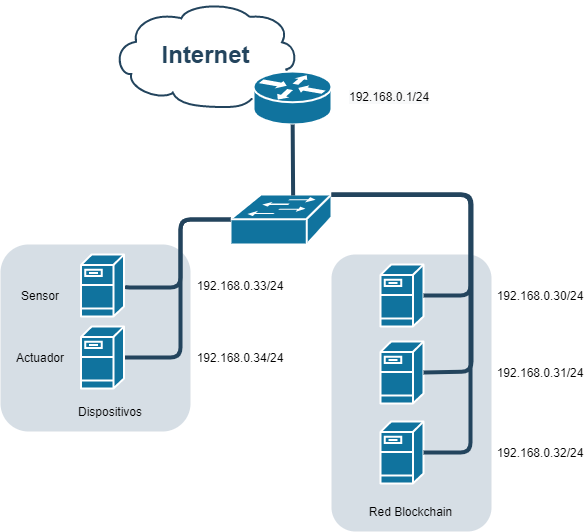
\includegraphics[width=0.7\textwidth]{imagenes/desarrollo/topologia_red}
  \caption{Topología de la red.}
  \label{fig:topologia-red}
\end{figure}

\begin{figure}[ht!]
  \centering
  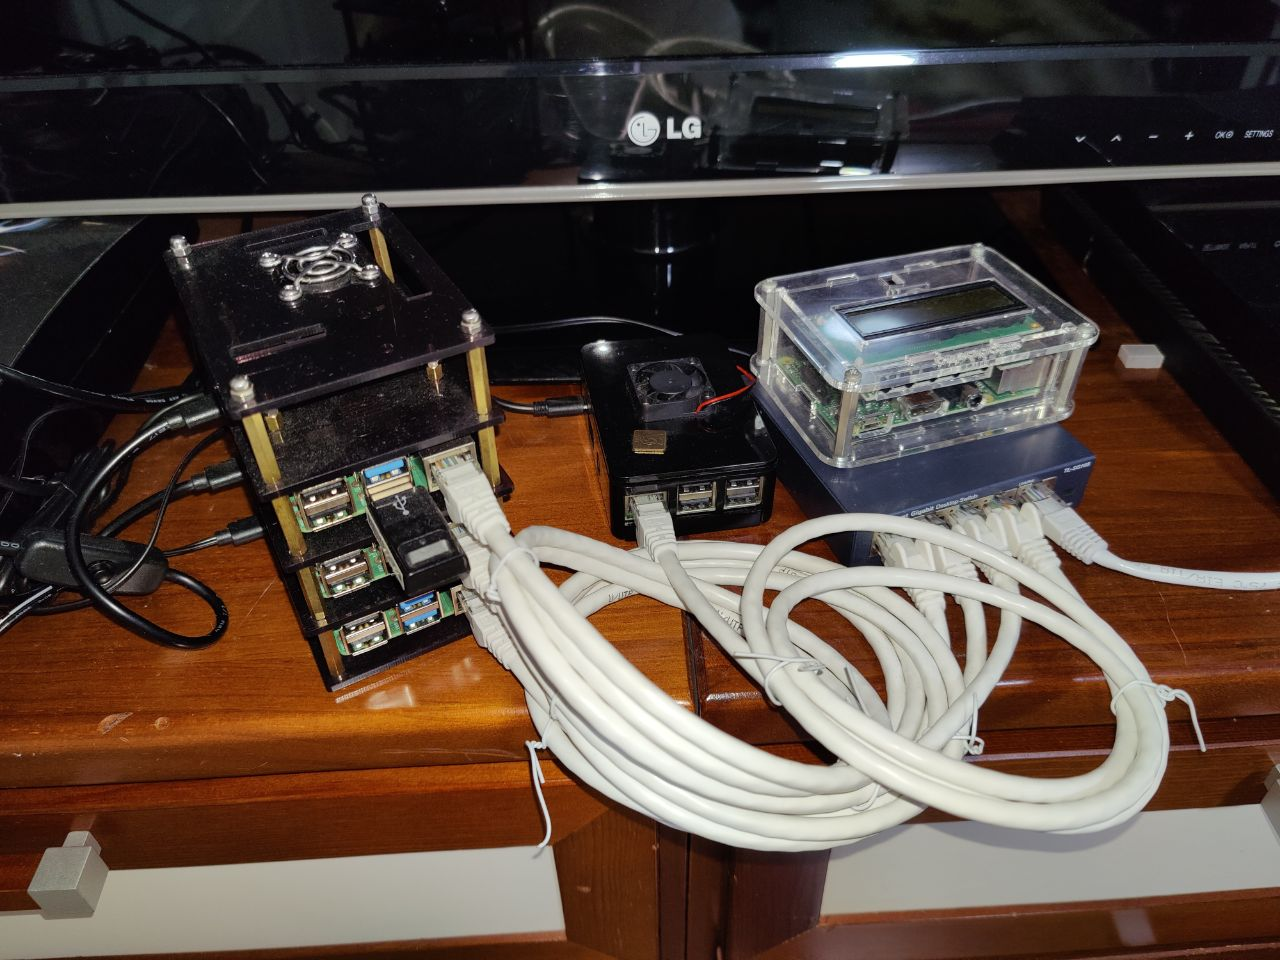
\includegraphics[width=0.7\textwidth]{imagenes/desarrollo/foto_raspberry}
  \caption{Captura de las Raspberry Pi.}
  \label{fig:captura-raspberry}
\end{figure}

\newpage

\subsubsection*{Instalación de Hyperledger Fabric 1.4.4.}

Para la instalación de Hyperledger Fabric (1.4.4) necesitaremos que cada nodo tengan los siguientes requisitos instalados 
\cite{hyperledger-fabric-docs}:

\begin{itemize}
  \item cURL.
  \item Docker version 17.06.2-ce o mayor \cite{install-docker-rasp, set-up-docker-rasp}.
  \item git.
  \item Docker Compose 1.14.0 o mayor \cite{install-docker-rasp, set-up-docker-rasp}.
  \item Go version 1.12.x
  \item Node.js
  \item npm version 5.6.0
  \item Python 2.7
\end{itemize}

\noindent Una vez instalado los requisitos procedemos a la creación de las imágenes de Hyperledger Fabric a partir de 
los binarios. Actualmente no hay soporte para arquitecturas ARM ya que Hyperledger solamente soporta las siguientes 
arquitecturas \cite{build-docker-images}:

\begin{itemize}
  \item amd64
  \item s390x
  \item ppc64le
\end{itemize}

\noindent Por tanto el principal objetivo y uno de los obstáculos importantes, era conseguir que Hyperledger Fabric 
se ejecutara en Raspberry Pi. Por ello, realice la construcción de mis propias imágenes de Docker que se pueden 
encontrar en mi DockerHub \cite{dockerhub}. Para ello, he tenido que realizar una serie de cambios en el código fuente
de Hyperledger Fabric que se encuentra distribuido en dos repositorios: \textbf{fabric-baseimage}\footnote{Actualmente, 
este proyecto se encuentra deprecated. \label{fnlabel}} y \textbf{fabric} \cite{fabric-baseimage, fabric}. 

\subsubsection*{fabric-baseimage}

Para poder llevar acabo la construcción de las imágenes Docker y los binarios, he forkeado el repositorio de 
Hyperledger/fabric-baseimage \cite{fabric-baseimage} desde la etiqueta v0.4.18 y he realizado los siguientes 
\href{https://github.com/Thejokeri/fabric-baseimage/commit/f3dfc7bcbdbd62c0c391aa3ce7eeb594ed6a3309}{cambios} para 
construir las imágenes con la última versión de arm64v8. Todos estos cambios se pueden encontrar en la rama \say{project} 
del repositorio \cite{fork-fabric-baseimage}.

\newpage

\noindent Clonamos el repositorio fork desde la rama proyect:

\begin{lstlisting}[language=bash]
  $ git clone -b project \ 
  https://github.com/Thejokeri/fabric-baseimage.git
\end{lstlisting}

\noindent Con la siguiente orden del Makefile:

\begin{lstlisting}[language=bash]
  $ make docker couchdb kafka zookeeper
\end{lstlisting}

\noindent generamos las imágenes necesarias:

\begin{itemize}
  \item fabric-baseos
  \item fabric-baseimage
  \item fabric-couchdb
  \item fabric-kafka
  \item fabric-zookeeper
\end{itemize}

\subsubsection*{fabric}

\noindent Desde el repositorio oficial, clonamos desde la rama v1.4.4:

\begin{lstlisting}[language=bash]
  $ git clone -b v1.4.4 https://github.com/hyperledger/fabric.git
\end{lstlisting}

\noindent Y lanzamos la siguiente orden Makefile, para generar las imágenes restantes de Hyperledger:

\begin{lstlisting}[language=bash]
  $ make native license spelling linter docker
\end{lstlisting}

\begin{itemize}
  \item fabric-tools
  \item fabric-buildenv
  \item fabric-ccenv
  \item orderer
  \item peer
\end{itemize}

\newpage

\noindent El resultado final es el siguiente:

\begin{figure}[ht!]
  \centering
  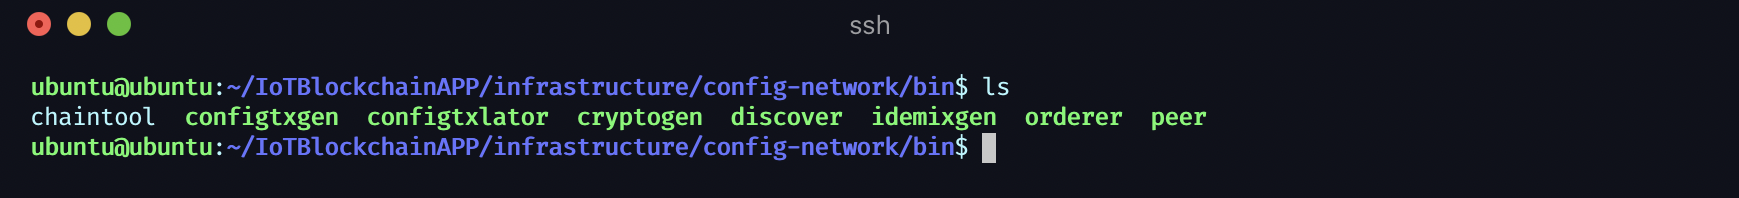
\includegraphics[width=\textwidth]{imagenes/desarrollo/binarios_fabric}
  \caption{Binarios de Hyperledger Fabric.}
  \label{fig:binarios-fabric}
\end{figure}

\begin{figure}[ht!]
  \centering
  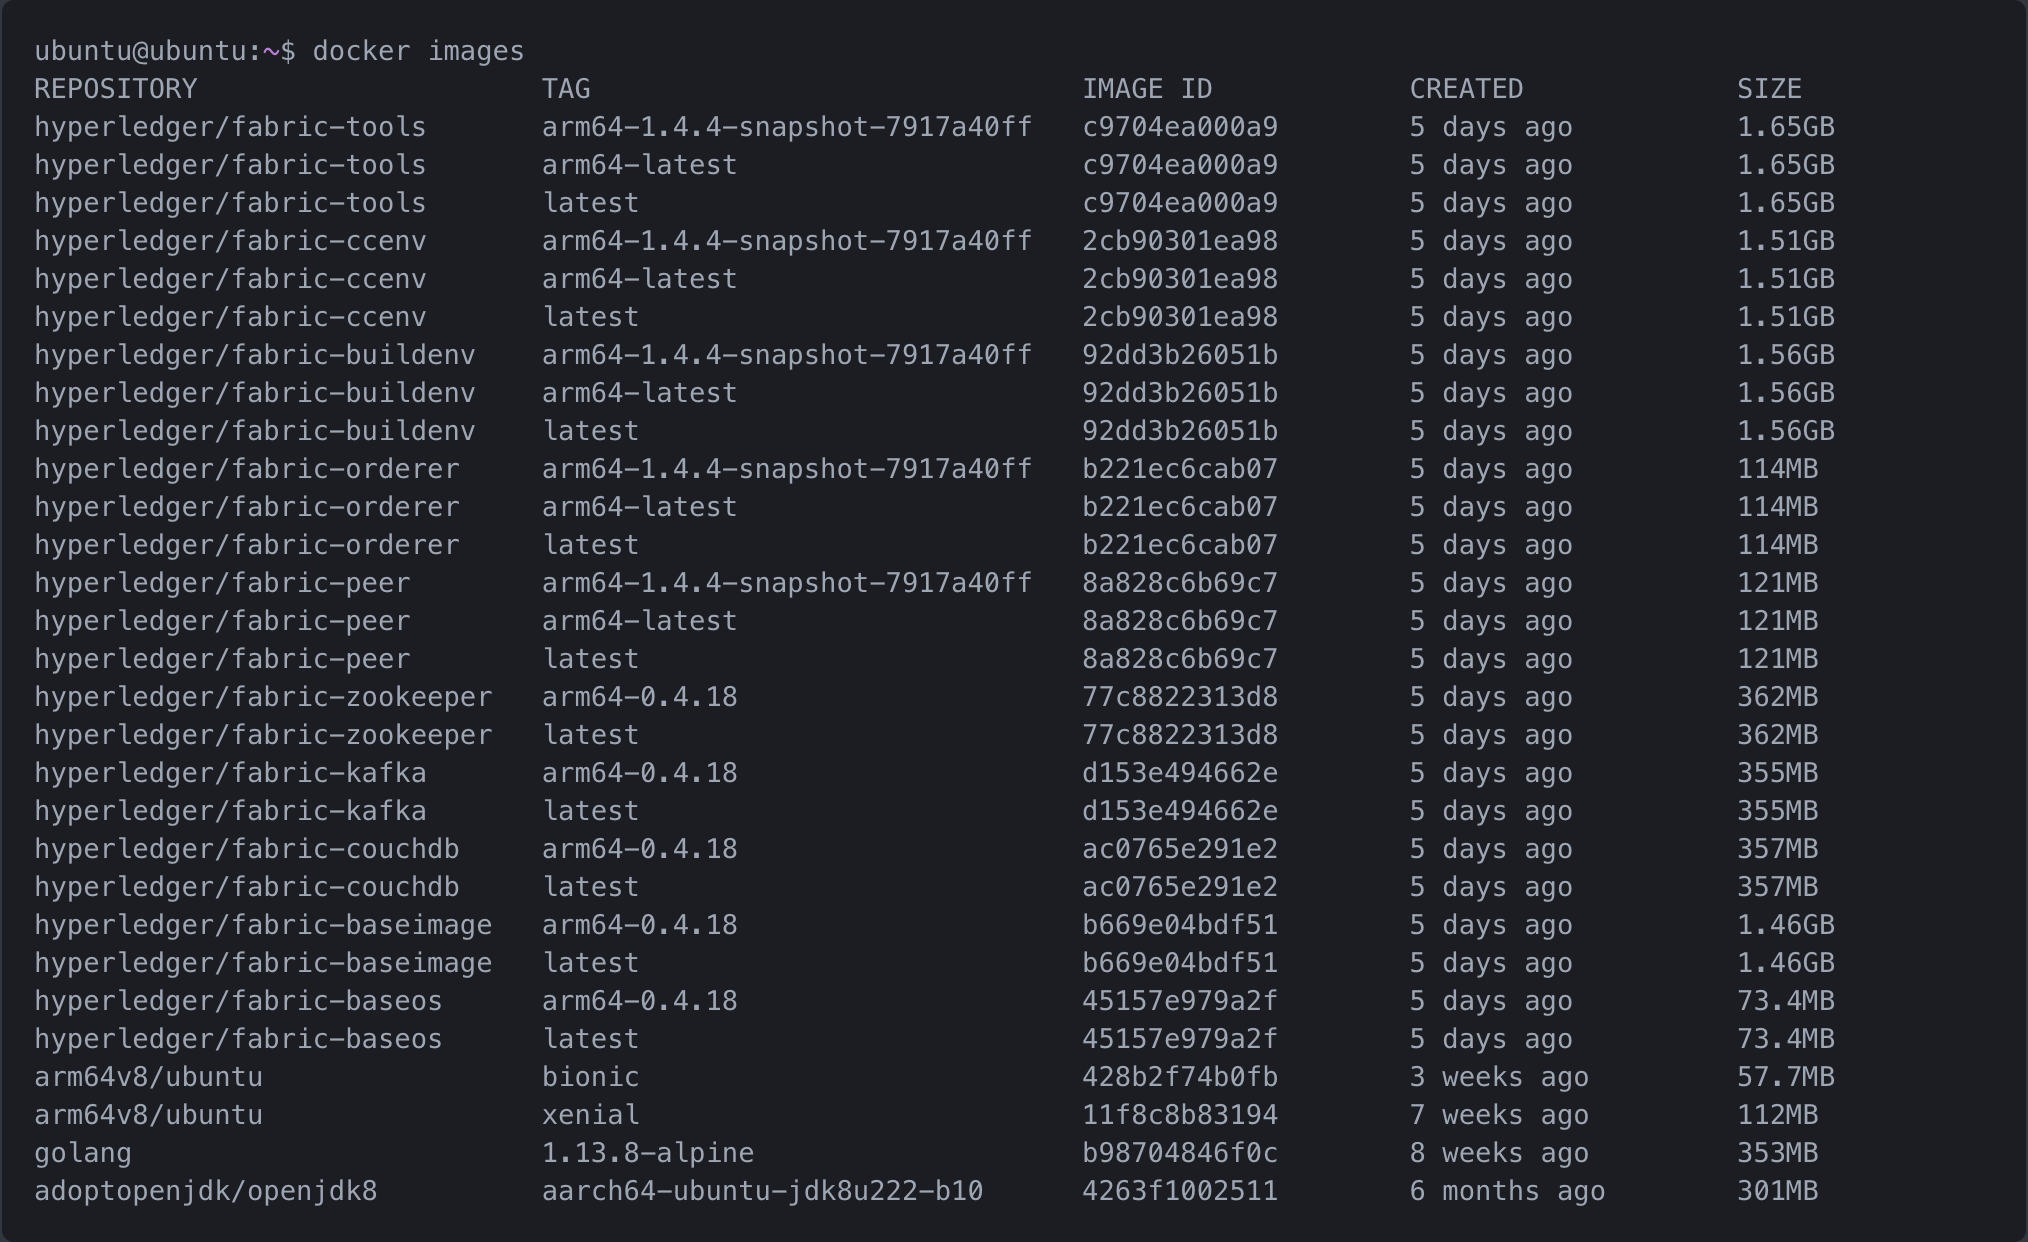
\includegraphics[width=\textwidth]{imagenes/desarrollo/imagenes_docker}
  \caption{Imágenes Docker de Hyperledger Fabric.}
  \label{fig:imagenes-docker}
\end{figure}

\noindent Como se mencionó anteriormente, vamos a utilizar varias Raspberry como nodos principales de la red 
Blockchain, voy a utilizar Docker Swarm para la orquestación de multiples contenedores dentro de múltiples 
máquinas anfitrionas. Para llevarlo a cabo, nos conectamos al nodo que va a ser el maestro, en este caso es la
máquina con IP \textbf{192.168.0.30}, e introducimos el siguiente comando:

\begin{lstlisting}[language=bash]
  $ docker swarm init
\end{lstlisting}

\noindent Este comando genera dos token al azar, una de trabajador y otra de gerente. Cuando unes un nuevo nodo al 
swarm, el nodo se une como un nodo trabajador o gerente basado en el token que usas para unirte al swarm.

\vspace{5mm}

\noindent Unimos los nodos \textbf{192.168.0.31} y \textbf{192.168.0.32} al swarm con el comando que se genera: 

\begin{lstlisting}[language=bash]
  $ docker swarm join --token SWMTKN-1-XXXX 192.168.0.30:2377
\end{lstlisting}

\newpage

\noindent En la siguiente figura podemos ver los nodos unidos y activos (ver fig. \ref{fig:node-ls-worker}):

\begin{figure}[ht!]
  \centering
  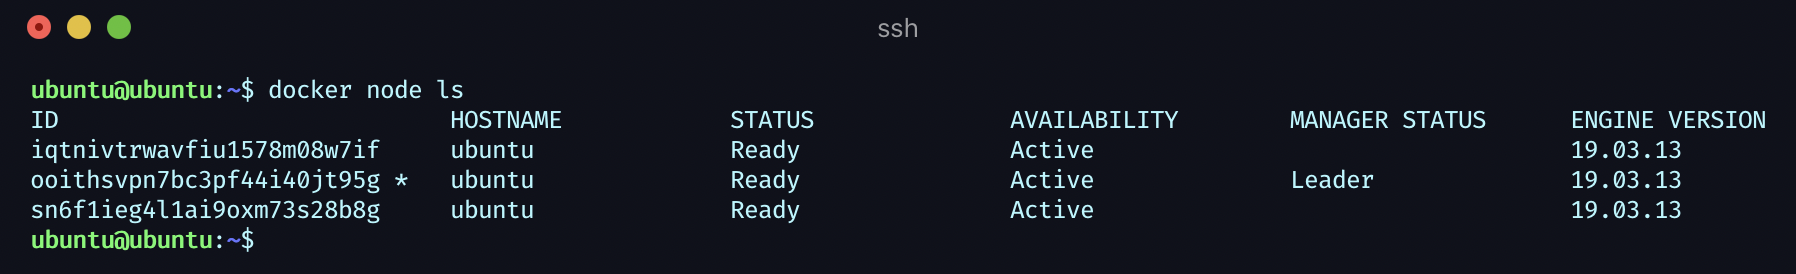
\includegraphics[width=\textwidth]{imagenes/desarrollo/comandos/node_ls_worker}
  \caption{Nodos de Docker Swarm.}
  \label{fig:node-ls-worker}
\end{figure}

\noindent Con Docker Swarm conseguimos que los contenedores que vayamos a crear para la red Blockchain, se lance de forma 
arbitraria en cada uno de los nodos y no nos tenemos que preocupar en ir levantando cada contenedor uno por uno
en las máquinas. Solamente basta con lanzarlo en el nodo maestro y él se encargará de asignarle los contenedores
a los nodos trabajadores activos, todo en una red privada \cite{hyperledger-fabric-rasp-swarm}.

\vspace{5mm}

\noindent Para facilitar el proceso de instalación de prerrequisitos, creación de binarios, imágenes, Docker Swarm, etc. 
Se ha creado un script \textbf{setup\_base.sh} que tiene las siguientes opciones:

\begin{lstlisting}[language=bash]
./setup_base.sh -h
Uso: setup_base.sh [opciones]

opciones:
-h : muestra esta ayuda
-p : instalar prerrequisitos
-f : instalar binarios e imagenes de Hyperlegder Fabric
-s : iniciar Docker Swarm cluster
-d : pull imagenes Docker
-w : muestra las versiones de los prerrequisitos

e.g. setup_base.sh -f
creara los binarios e imagenes de Hyperledger Fabric
\end{lstlisting}

\newpage

\subsection{Implementación de la red Blockchain.}

Después de configurar las Raspberry Pi e instalar los requisitos, vamos a implementar la red Blockchain.
Dentro del repositorio, la estructura de ficheros que rige la infraestructura de la red es la siguiente:

\begin{figure}[ht!]
  \centering
  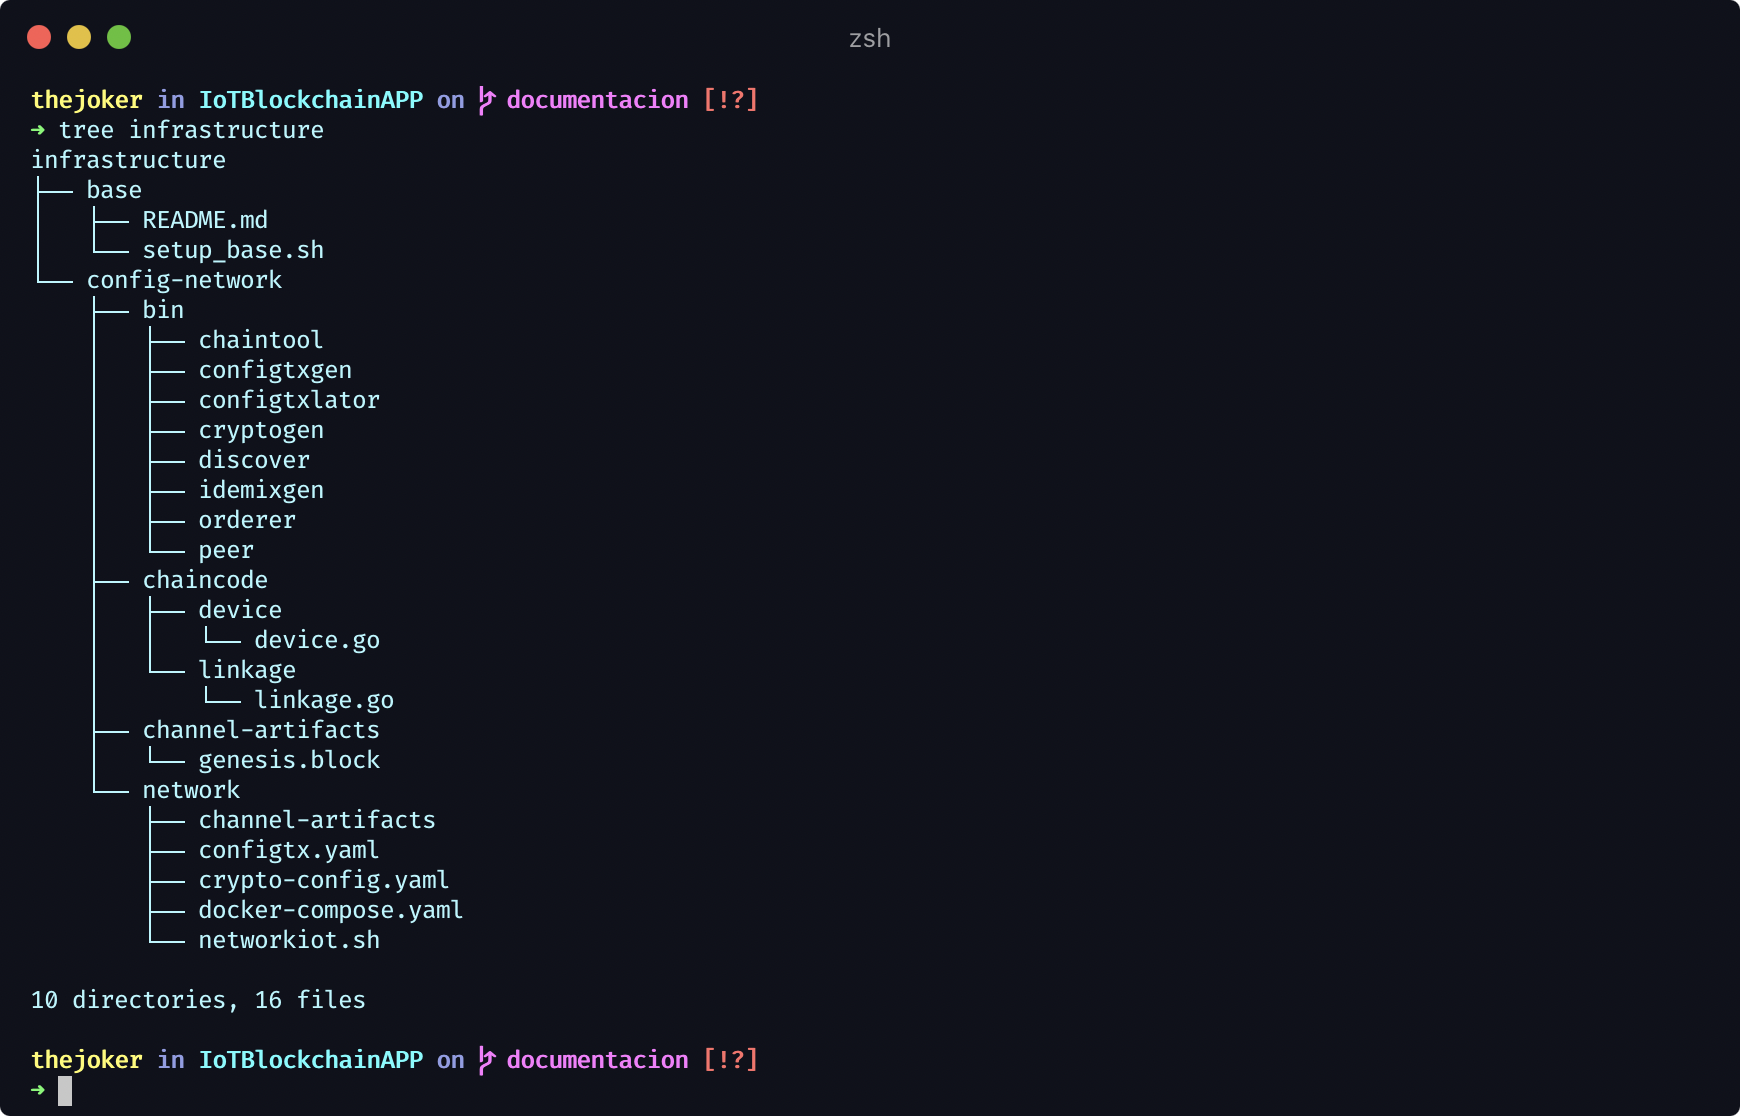
\includegraphics[width=\textwidth]{imagenes/desarrollo/tree_infraestructure}
  \caption{Tree de la carpeta infraestructure.}
  \label{fig:tree-infraestructure}
\end{figure}

\vspace{5mm}

\noindent La carpeta \textbf{config-network} contiene los binarios necesarios para las imágenes Docker de Hyperledger 
Fabric, los chaincode creados para realizar las operaciones a los dispositivos y enlaces 
\cite{developing-chaincode-nodejs}, y todos los ficheros necesarios para la configuración de la red Blockchain, que son: 

\begin{figure}[h!]
  \begin{subfigure}{0.5\textwidth}
    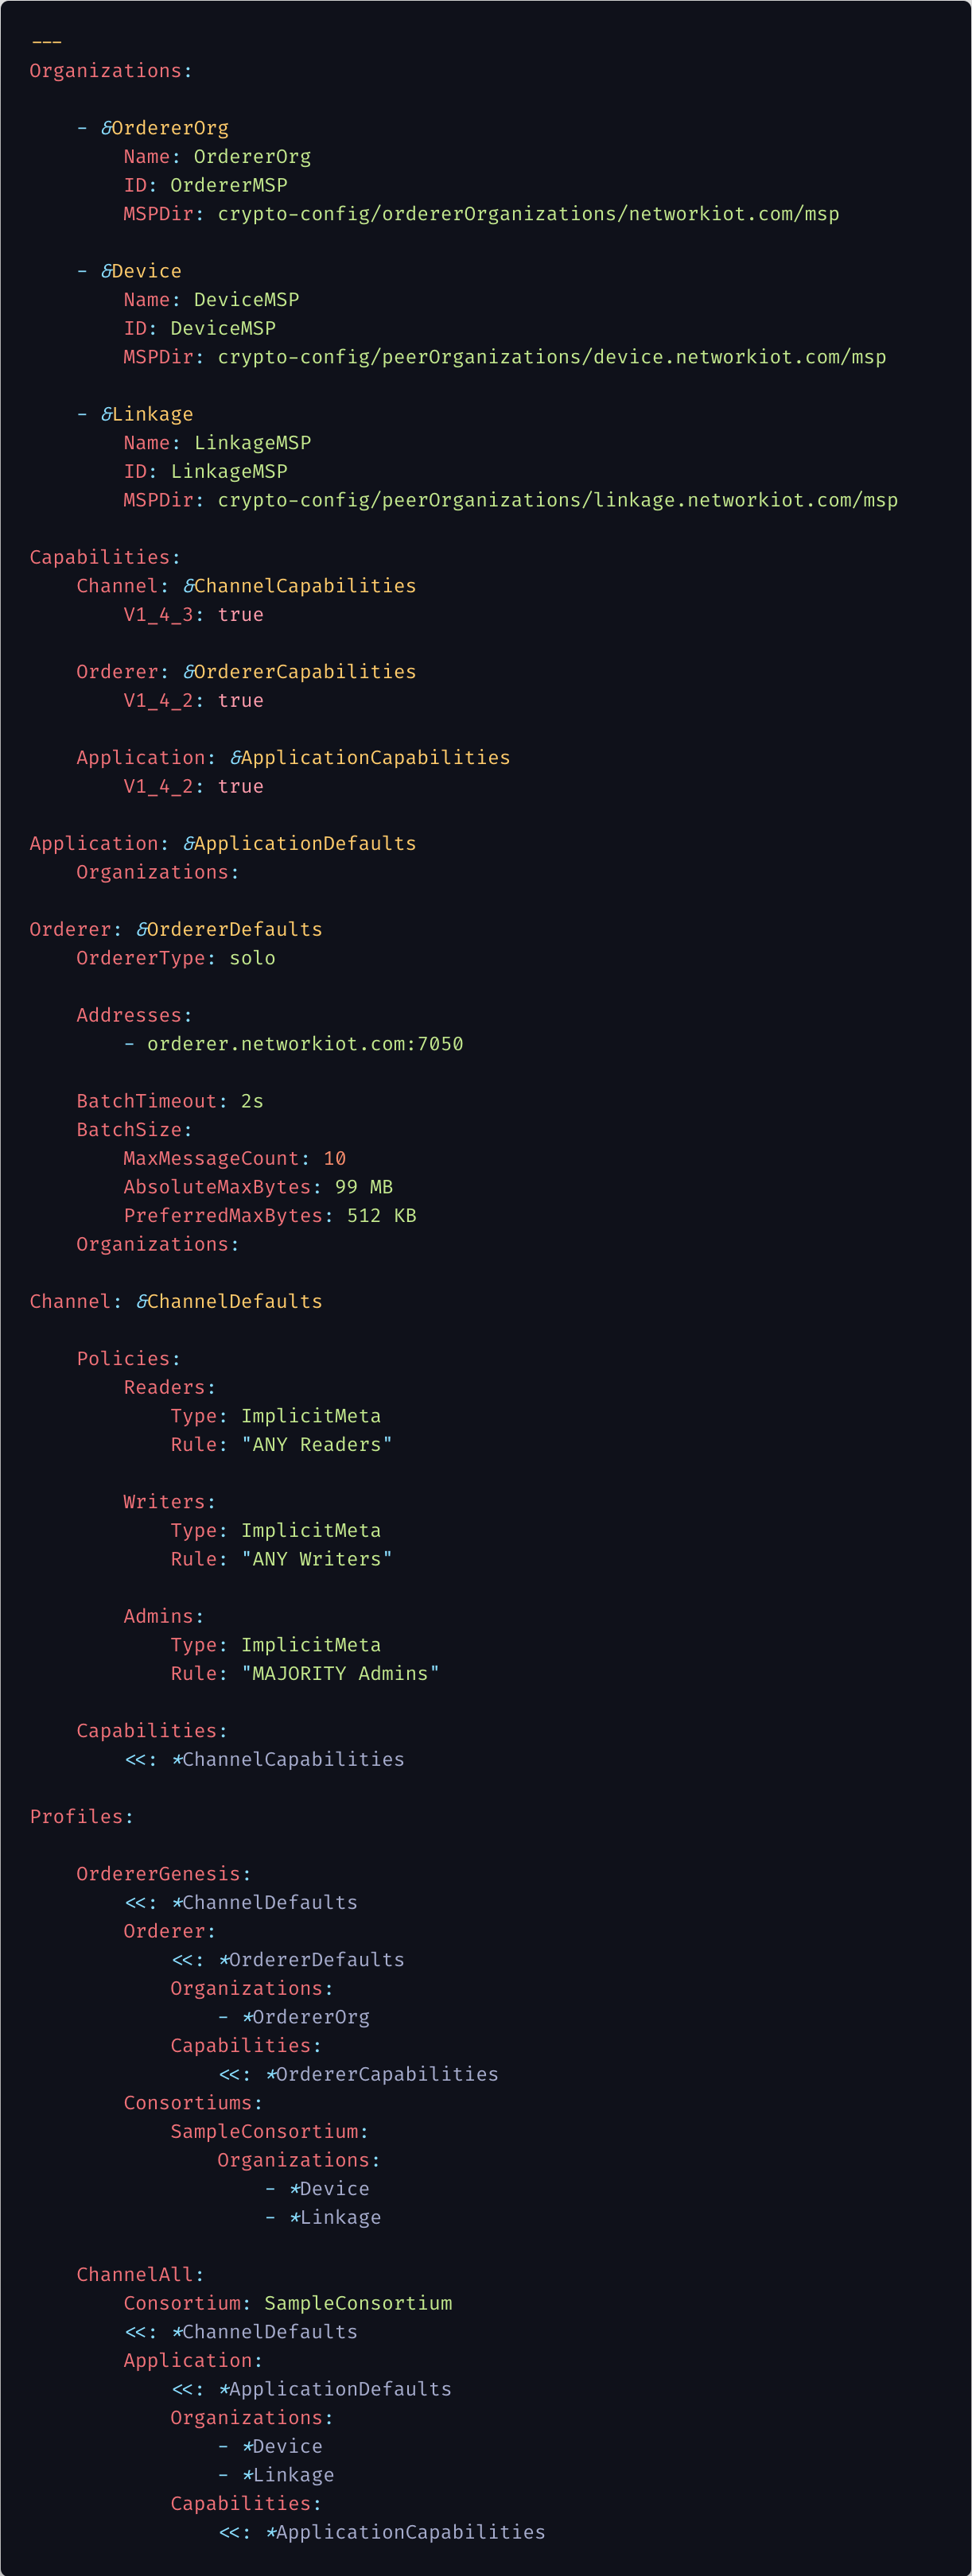
\includegraphics[width=\linewidth]{imagenes/desarrollo/configtx}
    \caption{Configtx de la red Blockchain.}
    \label{fig:configtx-blockchain}
  \end{subfigure}
  \begin{subfigure}{0.5\textwidth}
    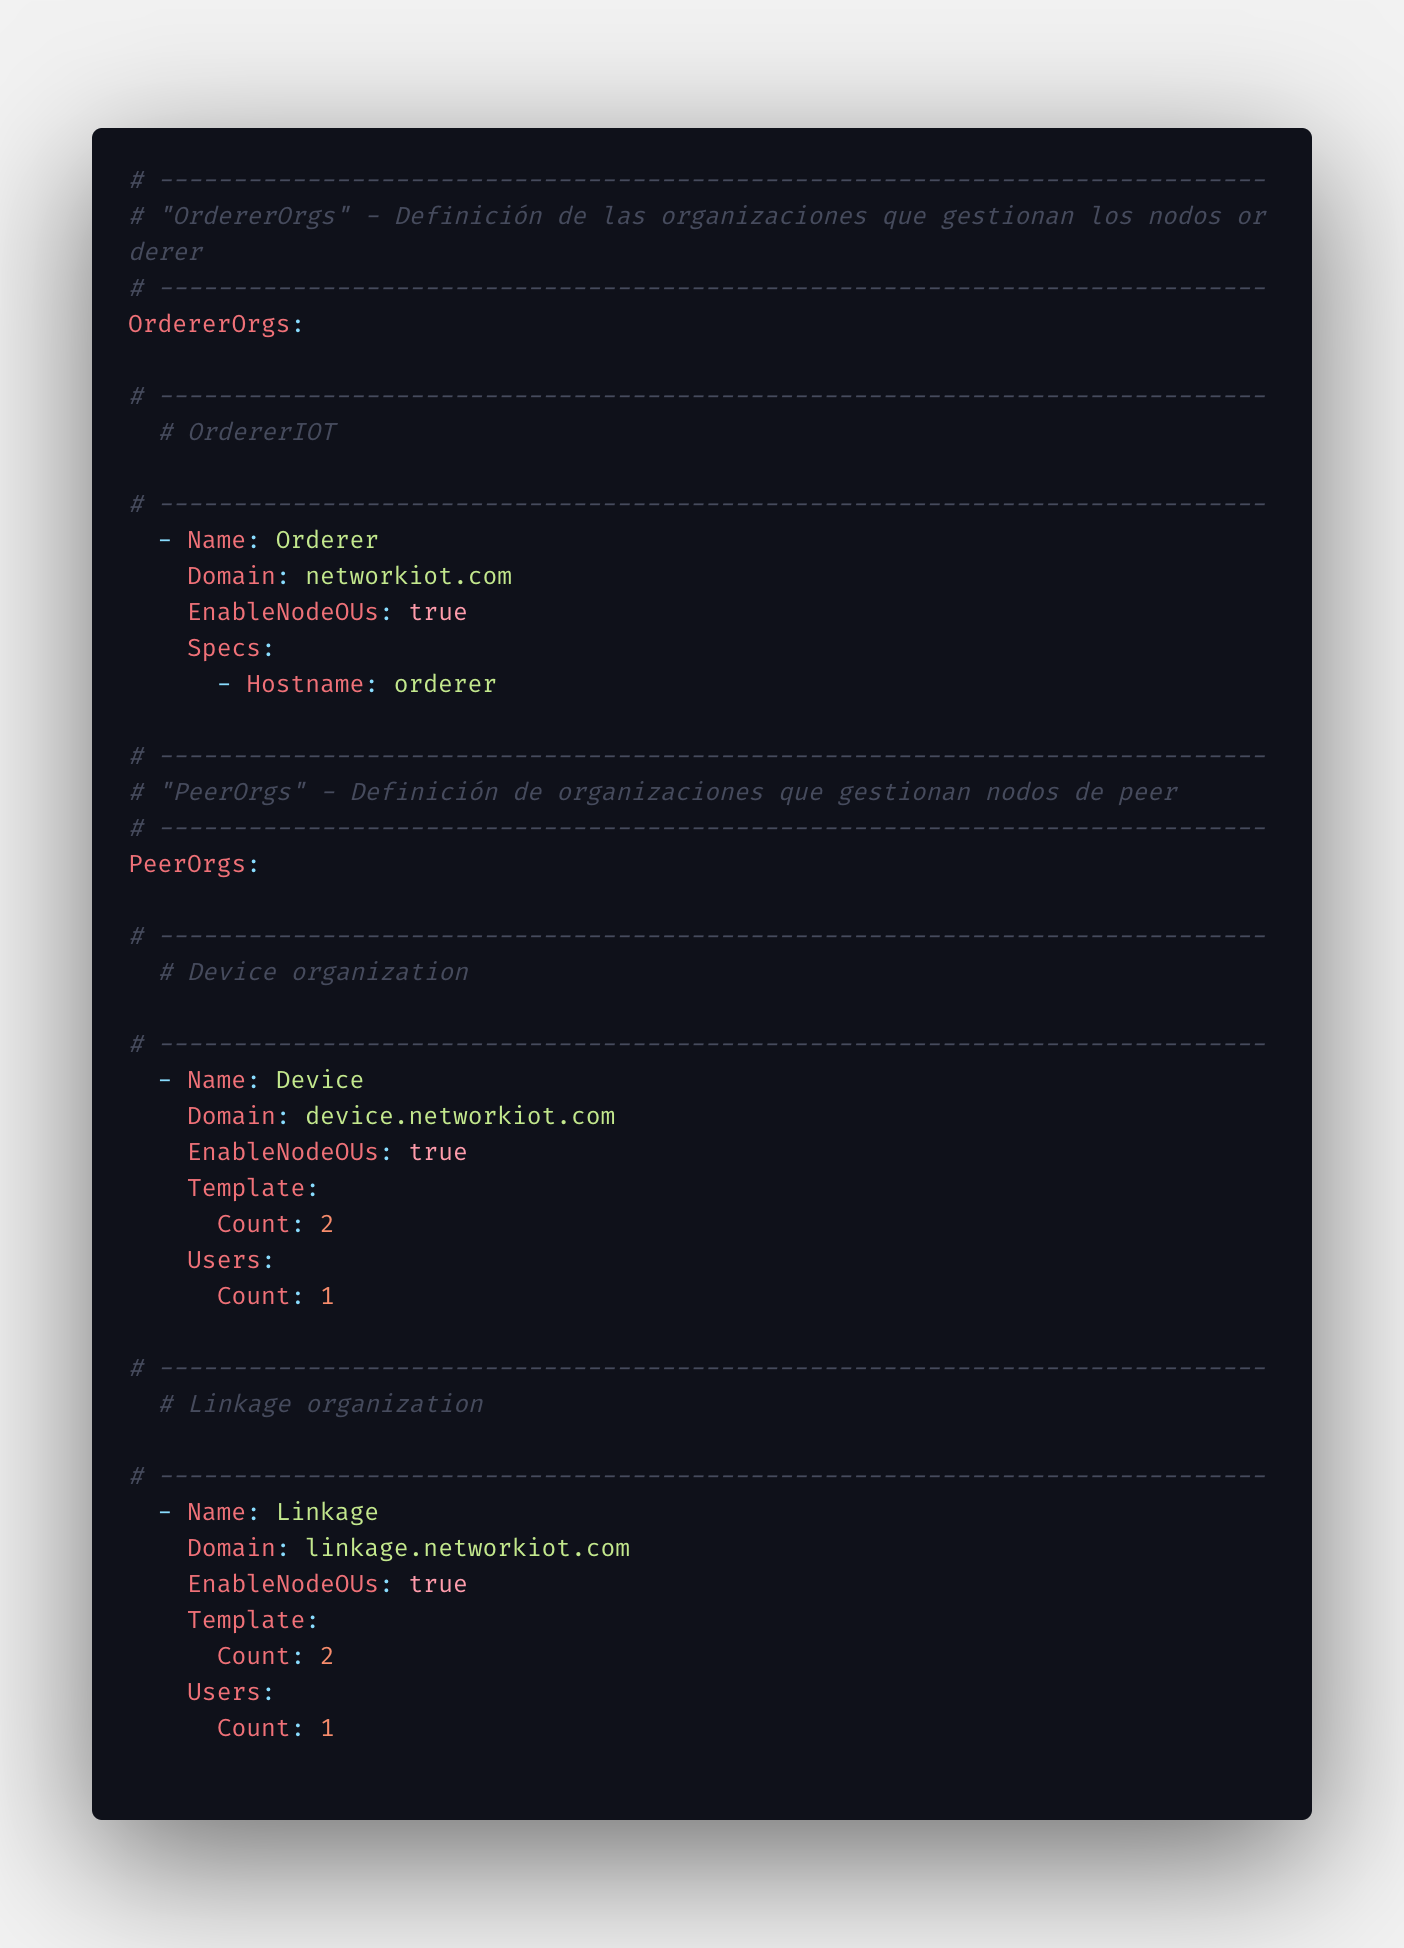
\includegraphics[width=\linewidth]{imagenes/desarrollo/crypto-config}
    \caption{Crypto-config de la red Blockchain.}
    \label{fig:crypto-config-blockchain}
  \end{subfigure}
  \caption{ficheros de configuración de la red Blockchain.}
  \label{fig:config-file-blockchain}
\end{figure}

\newpage

\noindent El fichero crypto-config se divide en dos secciones, las organizaciones orderer y las organizaciones peer. 
Para esta arquitectura hemos escogido una organización orderer con host \textbf{orderer.networkiot.com} y dos 
organizaciones peer con host \textbf{device.networkiot.com} y \textbf{linkage.networkiot.com}. 

\vspace{10mm}

\noindent Por otra parte, el fichero configtx se estructura en varias secciones, tenemos organizaciones, orderers,  
aplicaciones, capacidades y perfiles. Las secciones que podemos destacar son las organizaciones que van a formar la red 
Blockchain, en este caso tenemos una organización orderer y dos organizaciones peer: \textbf{Device} y \textbf{Linkage}. 
Por otro lado, tenemos los perfiles donde indicamos cuales organizaciones pertenecen a la organización orderer y canales, 
en este caso en el archivo indicamos que el único canal que vamos a crear, llamado \textbf{ChannelAll}, van a poder 
comunicarse los peers pertenecientes a la organización Device o Linkage.

\vspace{5mm}

\noindent Cabe destacar el documento \textbf{docker-compose.yaml}, en el se indican los contenedores que se va a lanzar 
para formar la red blockchain, que variables de entorno van a tener cada uno, en que nodos se van a lanzar y la red 
privada en la que se van a encontrar. Dentro del fichero vamos a encontrar un nodo orderer y un CLI para realizar 
consultas directamente a la red, luego dos parejas de nodos peer por cada organización que hay (Device y Linkage), 
cuatro bases de datos CouchDB para cada nodo peer y dos entidades certificadoras. Para ilustrar mejor la arquitectura de 
la red Blockchain (ver fig. \ref{fig:arquitectura-blockchain}). Los nodos orderer y CLI se van a lanzar en la máquina 
maestro y el resto se van a administrar en las otras dos máquinas trabajadoras.

\begin{figure}[h!]
  \centering
  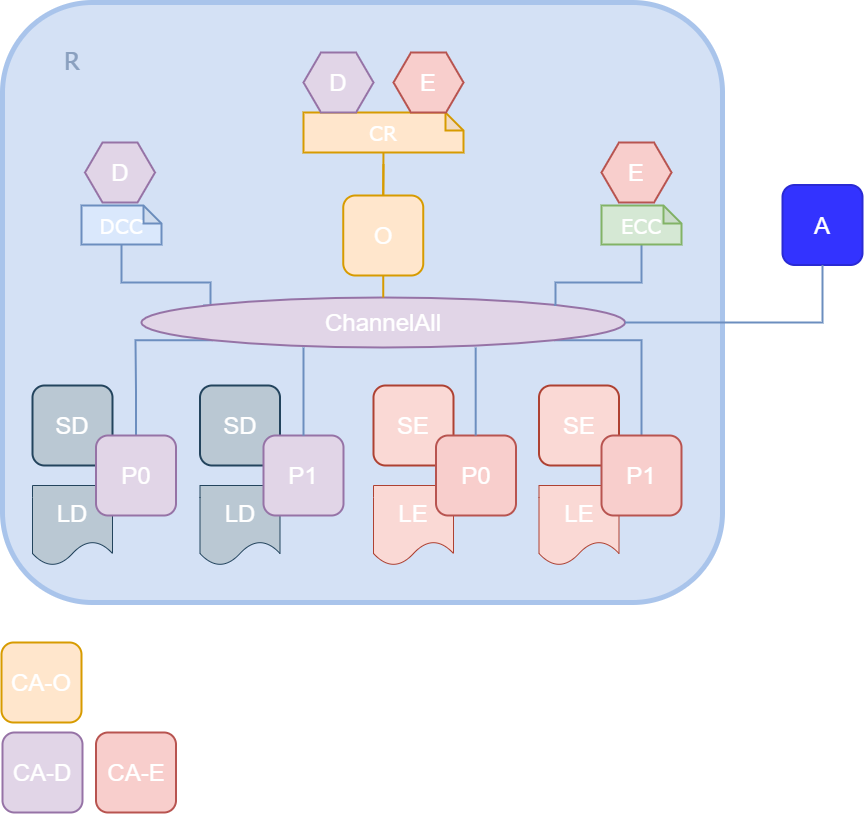
\includegraphics[width=\textwidth]{imagenes/desarrollo/arquitectura_networkiot}
  \caption{Arquitectura de la red Blockchain.}
  \label{fig:arquitectura-blockchain}
\end{figure}

\noindent Se ha elaborado un script, \textbf{networkiot.sh}, para automatizar el proceso de generación de la red, la 
orquestación de los contenedores, la creación y copia de los certificados y ficheros necesarios a cada una de las 
máquinas y la instalación y el proceso de instanciar de los chaincode. Incluso se ha añadido el comando para la 
eliminación de la red. \cite{byfn, deploy-stack-swarm}

\vspace{5mm}

\begin{lstlisting}[language=bash]
./networkiot.sh help
Uso: networkiot.sh [help, up, down, generate, restart, remove]

Comandos:
  help        Mostrar esta ayuda
  up          Activar red
  generate    Generar red
  remove      Eliminar red
  all         Generar y Activar red
\end{lstlisting}

\begin{figure}[ht!]
  \centering
  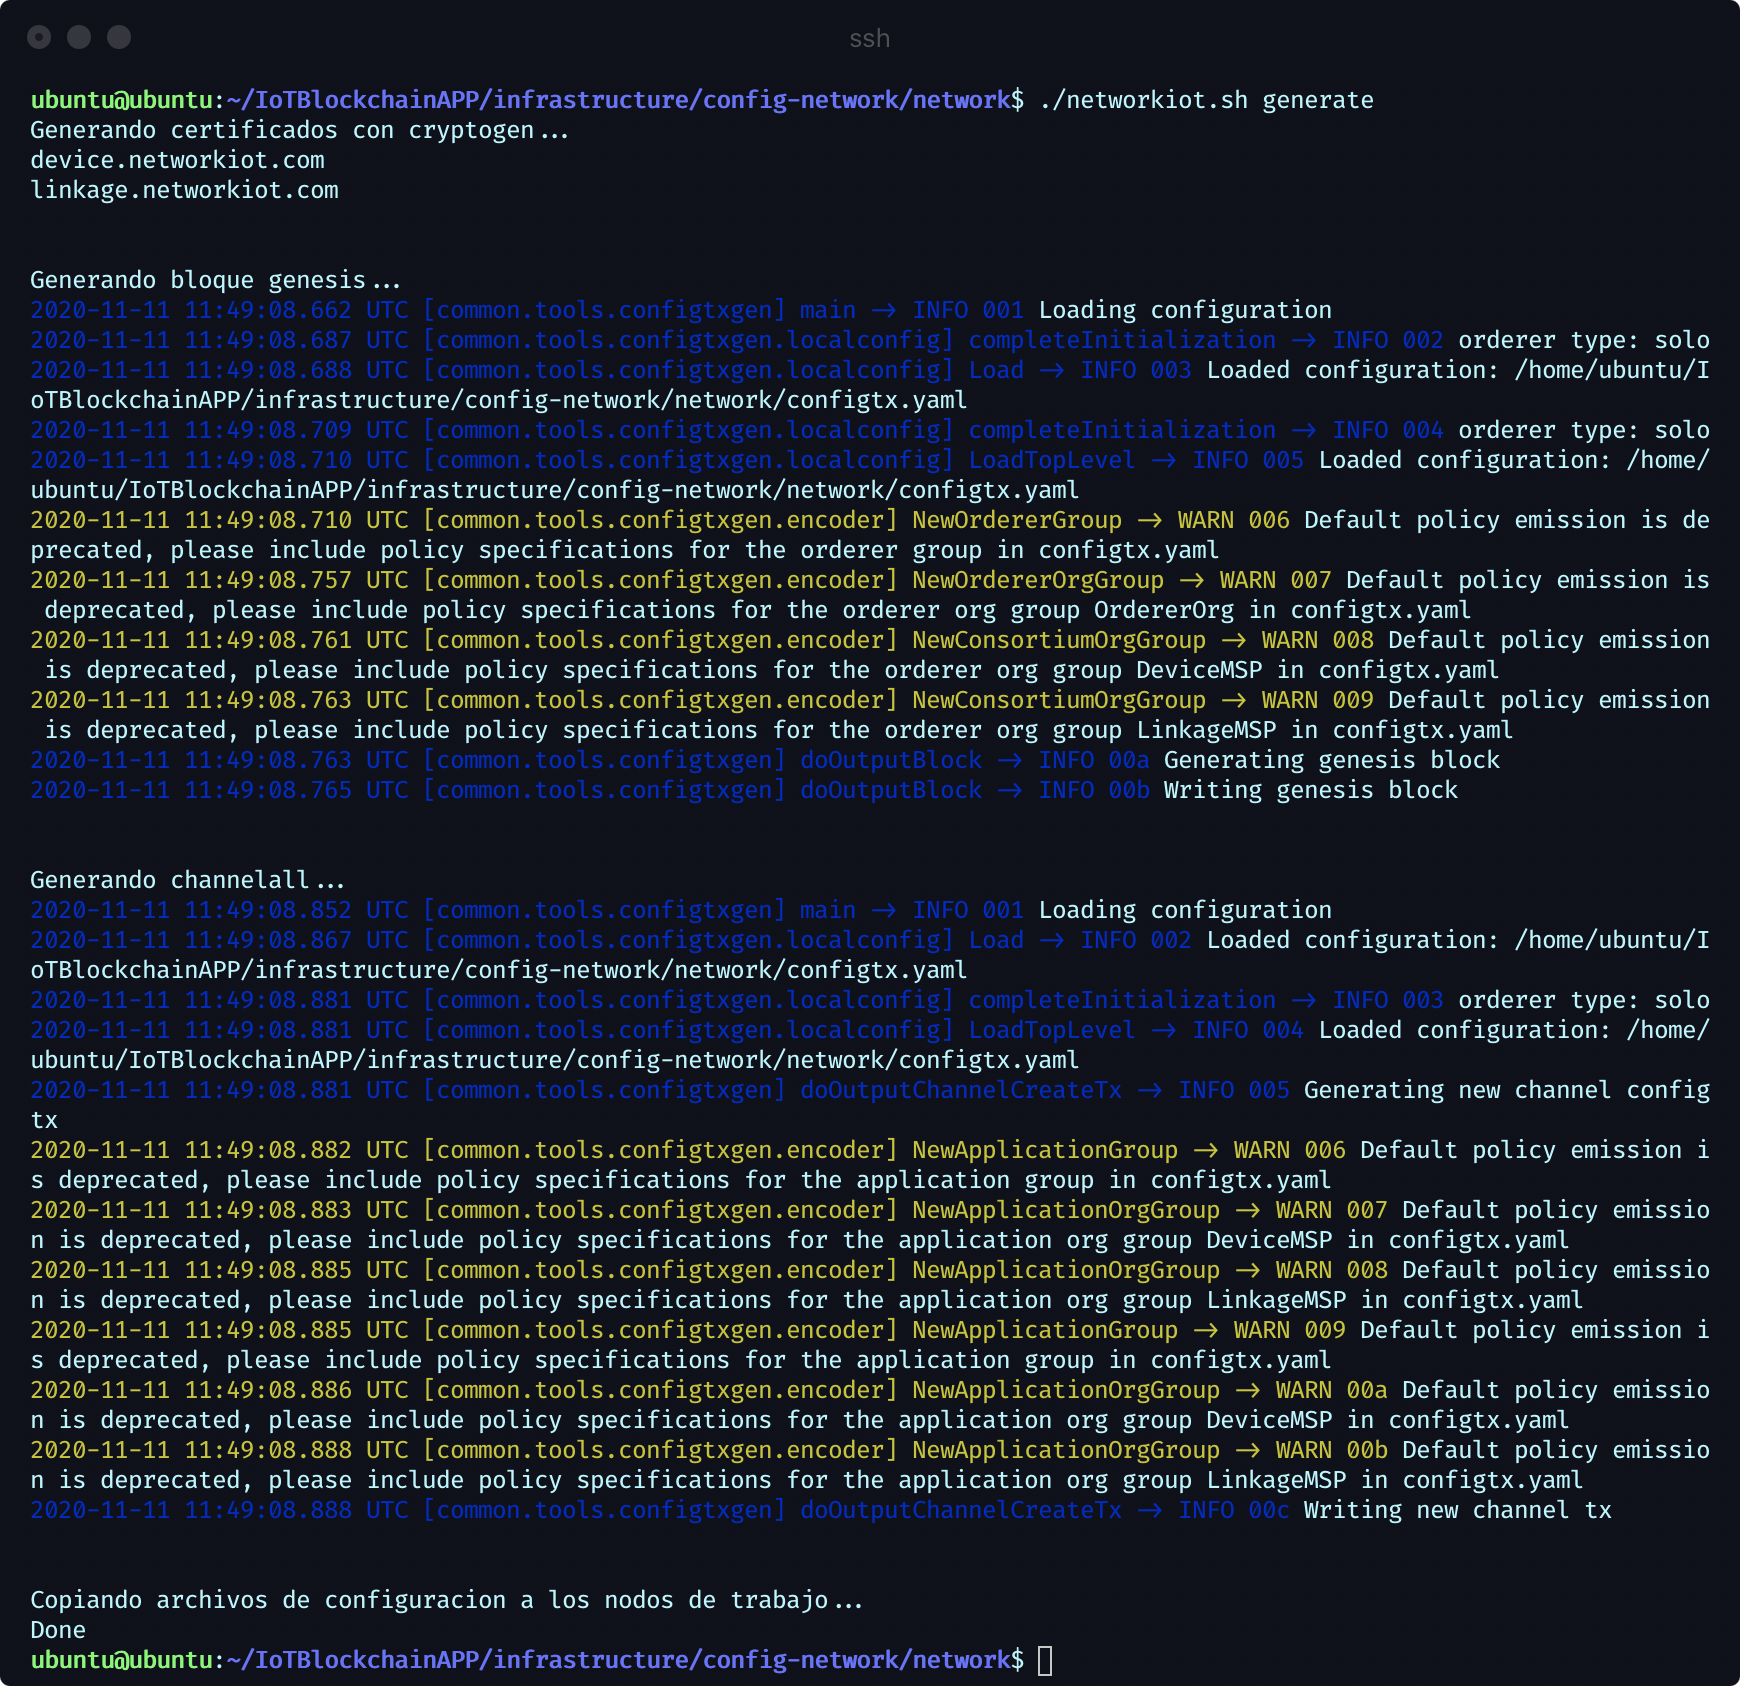
\includegraphics[width=\textwidth]{imagenes/desarrollo/comandos/generate}
  \caption{Opción generate del script networkiot.}
  \label{fig:generate}
\end{figure}

\noindent Al lanzar el comando \textbf{generate} en el nodo maestro, se creará la carpeta channel-artifacts que 
guardarán los archivos generados por el binario \textbf{cryptogen}, que es usado para la creación de los archivos de la 
red, pasandole como parámetro el archivo de configuración \textbf{crypto-config}. Los archivos que se generan son:

\begin{itemize}
  \item channel.tx: archivo para la transacción de configuración del canal.
  \item genesis.block: es el primer bloque de la cadena, el bloque génesis, el cual inicia la cadena de bloques de 
  nuestra red.
\end{itemize}

\noindent También se creará la carpeta crypto-config, que guardará las credenciales de nuestra red Hyperledger Fabric, 
para que se puedan conectar los diferentes usuarios y aplicaciones, tanto del ordenante como de todos los 
participantes. Las credenciales tienen que estar disponibles en todos los nodos y han de ser las mismas. Por tanto, se 
realiza una copia tanto de la carpeta channel-artifacts como crypto-config, a las otras máquinas que forman la red.

\vspace{5mm}

\noindent Ahora toca lanzar el comando \textbf{up}, que se encargará de:

\begin{itemize}
  \item Crear los certificados de los CA y compartirlos con las otras máquinas.
  \item Crear la red privada \textbf{networkiot} para los contenedores.
  \item Levantar los contenedores y los servicios Docker.
  \item Crear el canal \textbf{ChannelAll} e unir los nodos peer al canal.
  \item Instalar e instanciar los chaincode en el canal.
\end{itemize}

\begin{figure}[h!]
  \begin{subfigure}{0.5\textwidth}
    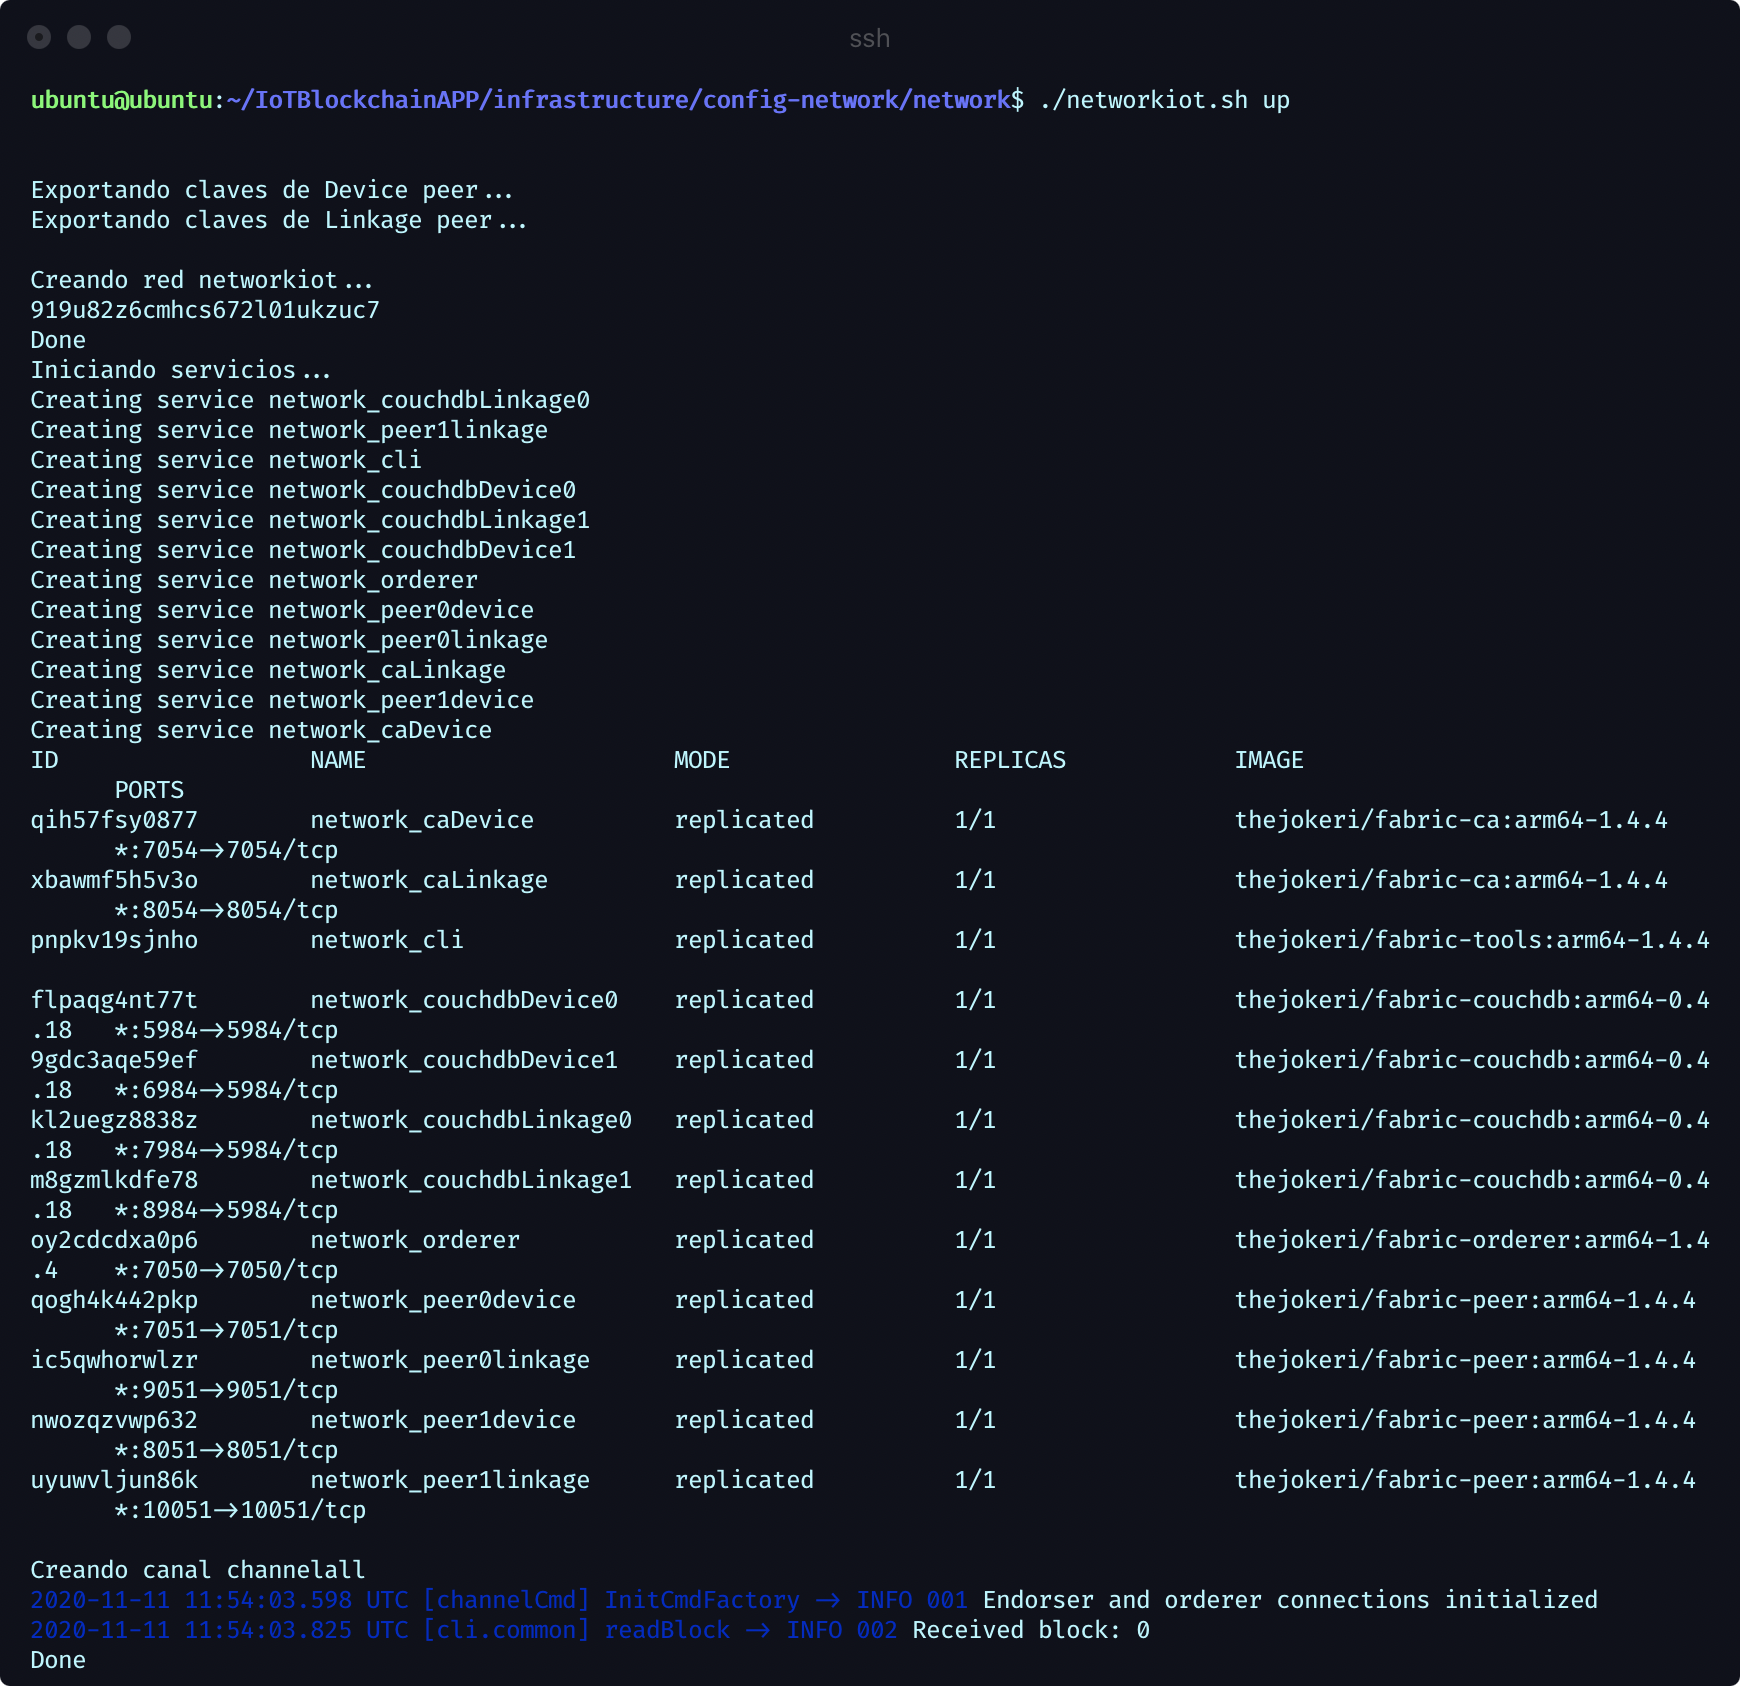
\includegraphics[width=\linewidth]{imagenes/desarrollo/comandos/up_1}
    \caption{Salida 1 de la opción up del script networkiot.}
    \label{fig:up-1}
  \end{subfigure}
  \begin{subfigure}{0.5\textwidth}
    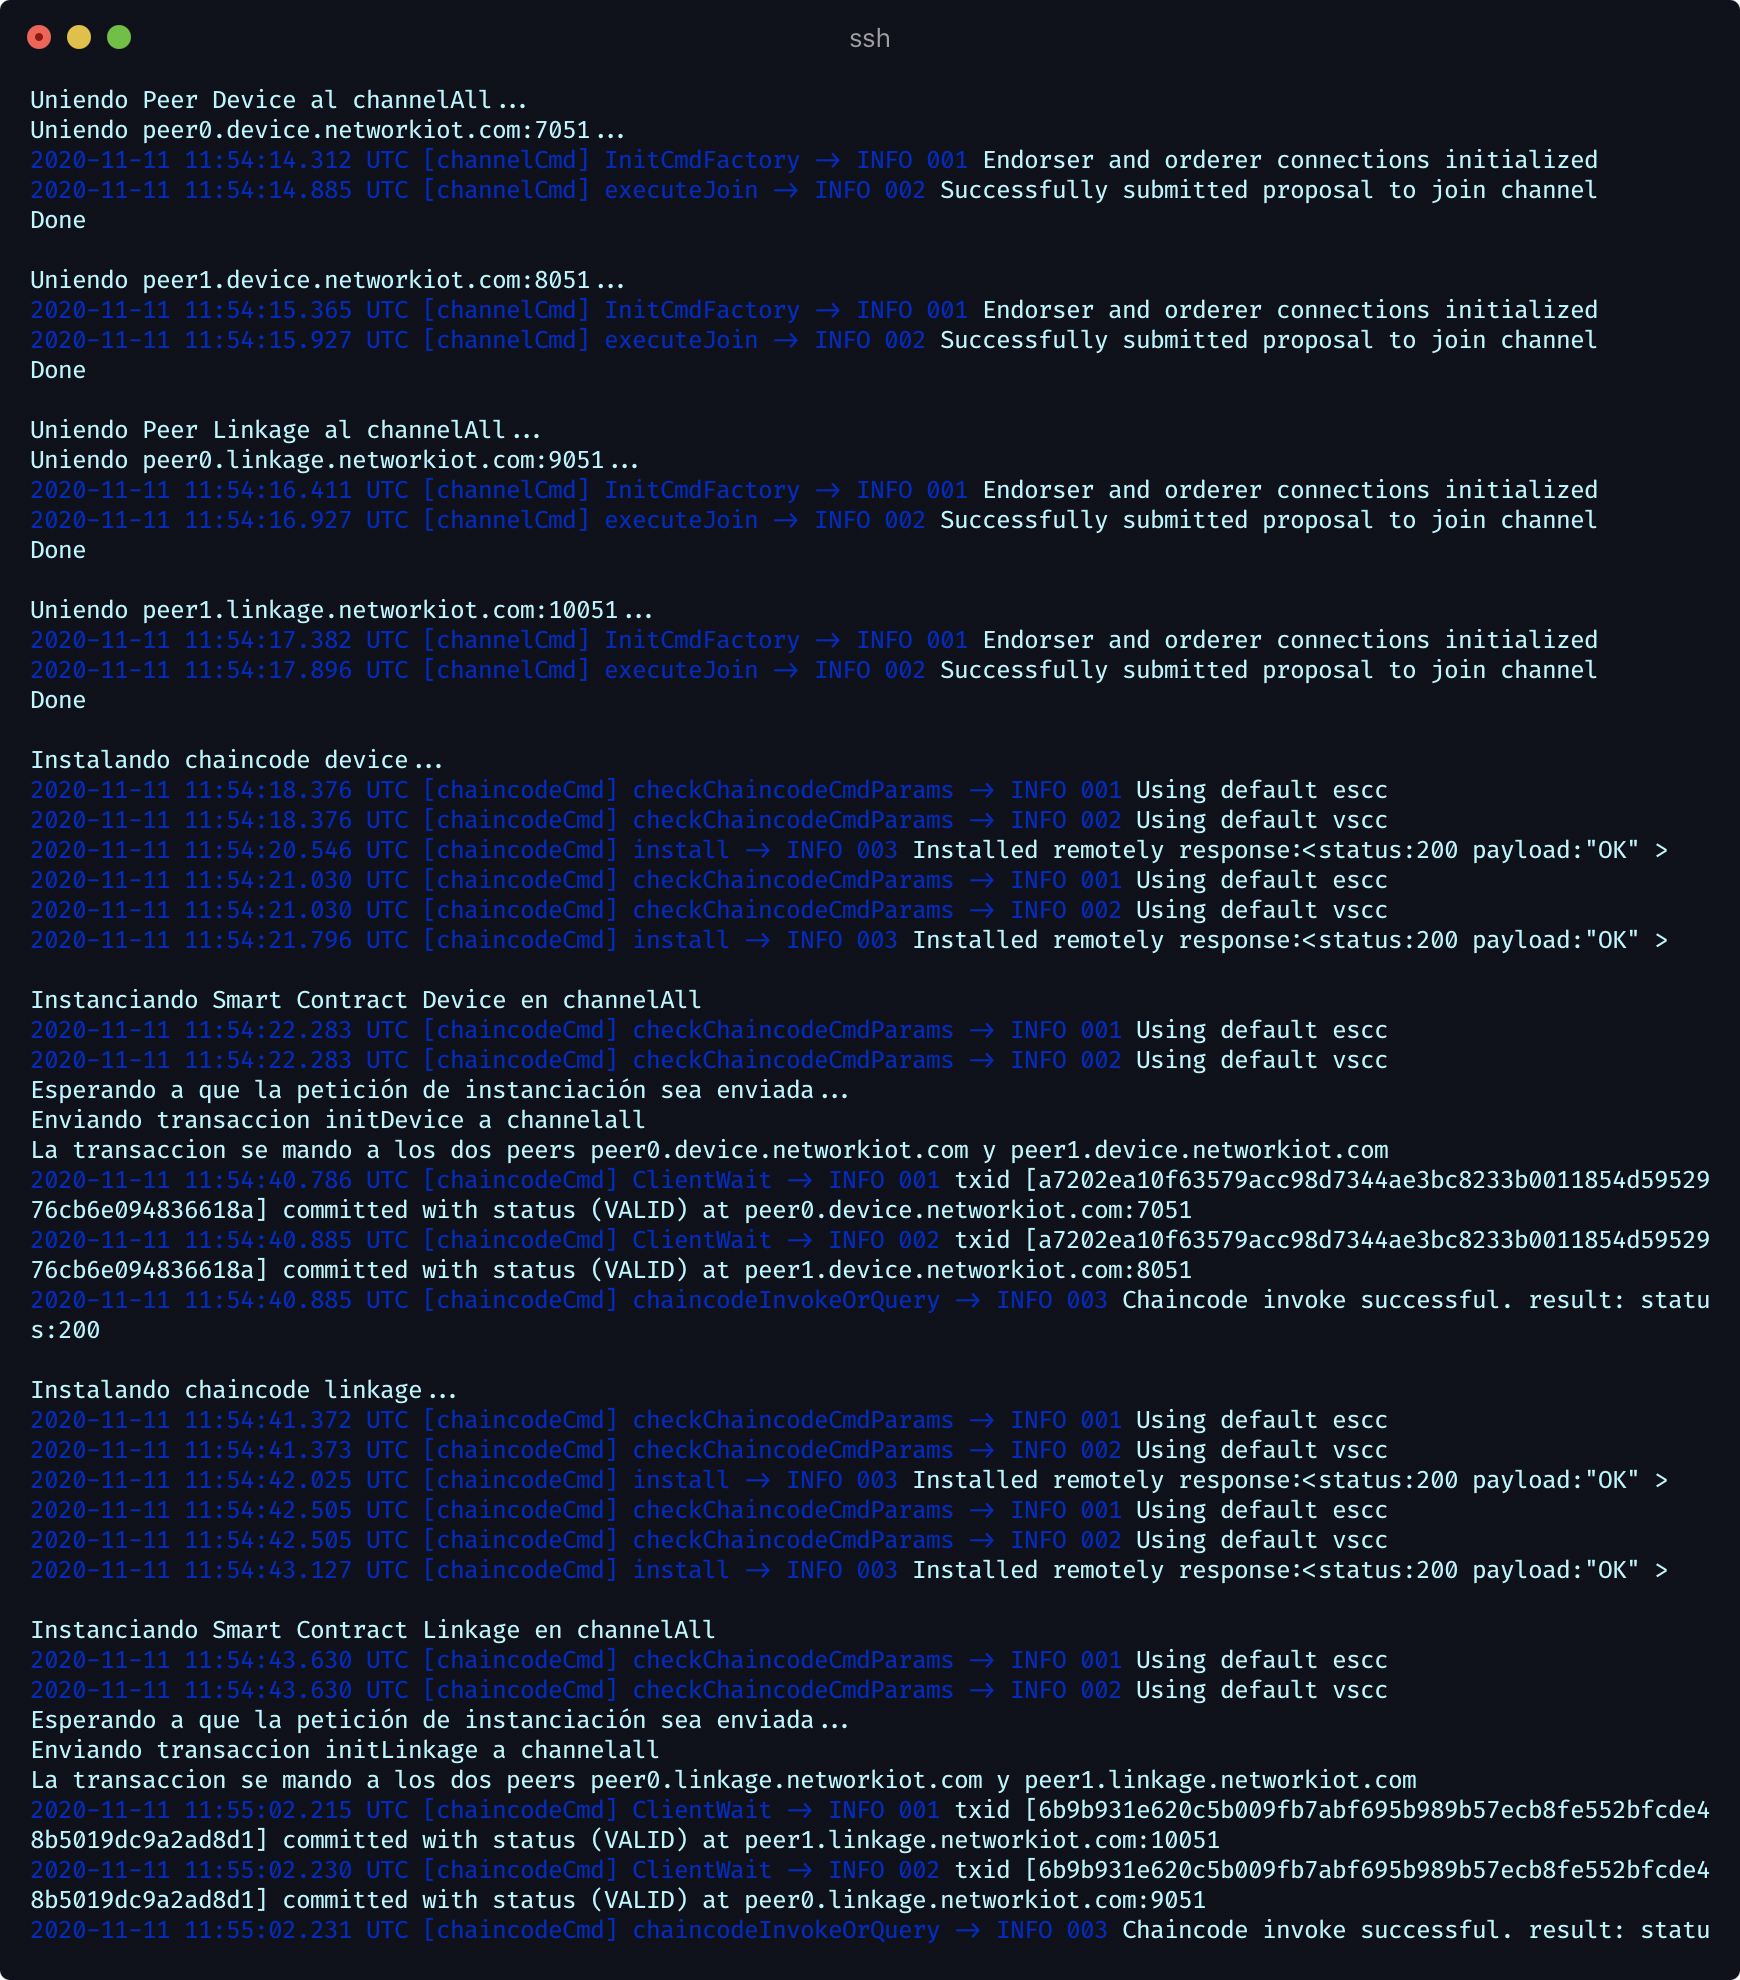
\includegraphics[width=\linewidth]{imagenes/desarrollo/comandos/up_2}
    \caption{Salida 2 de la opción up del script networkiot.}
    \label{fig:up-2}
  \end{subfigure}
  \caption{Salidas del comando up.}
  \label{fig:up}
\end{figure}

\noindent Este proceso es el más importante para la creación de la red Blockchain. A continuación vamos a mostrar los 
servicios y los contenedores que se han creado. Vamos a poder comprobar como Docker Swarm se ha encargado de gestionar 
la administración de los contenedores en cada uno de las máquinas.

\begin{figure}[ht!]
  \centering
  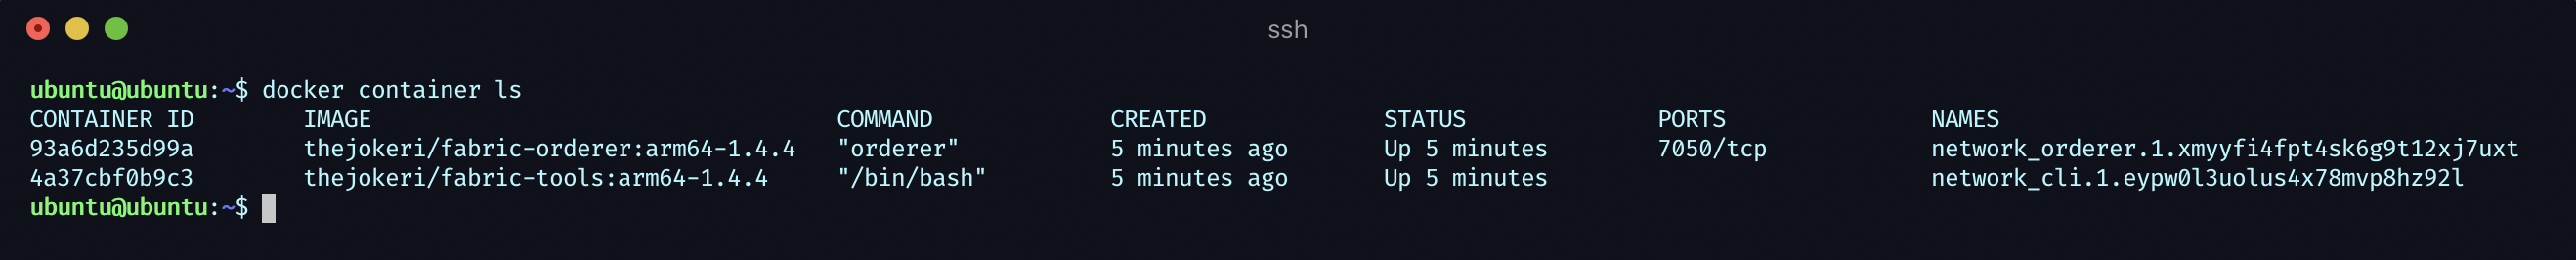
\includegraphics[width=\textwidth]{imagenes/desarrollo/comandos/containers_master}
  \caption{Salida de contenedores en el nodo maestro.}
  \label{fig:containers-master}
\end{figure}

\begin{figure}[ht!]
  \centering
  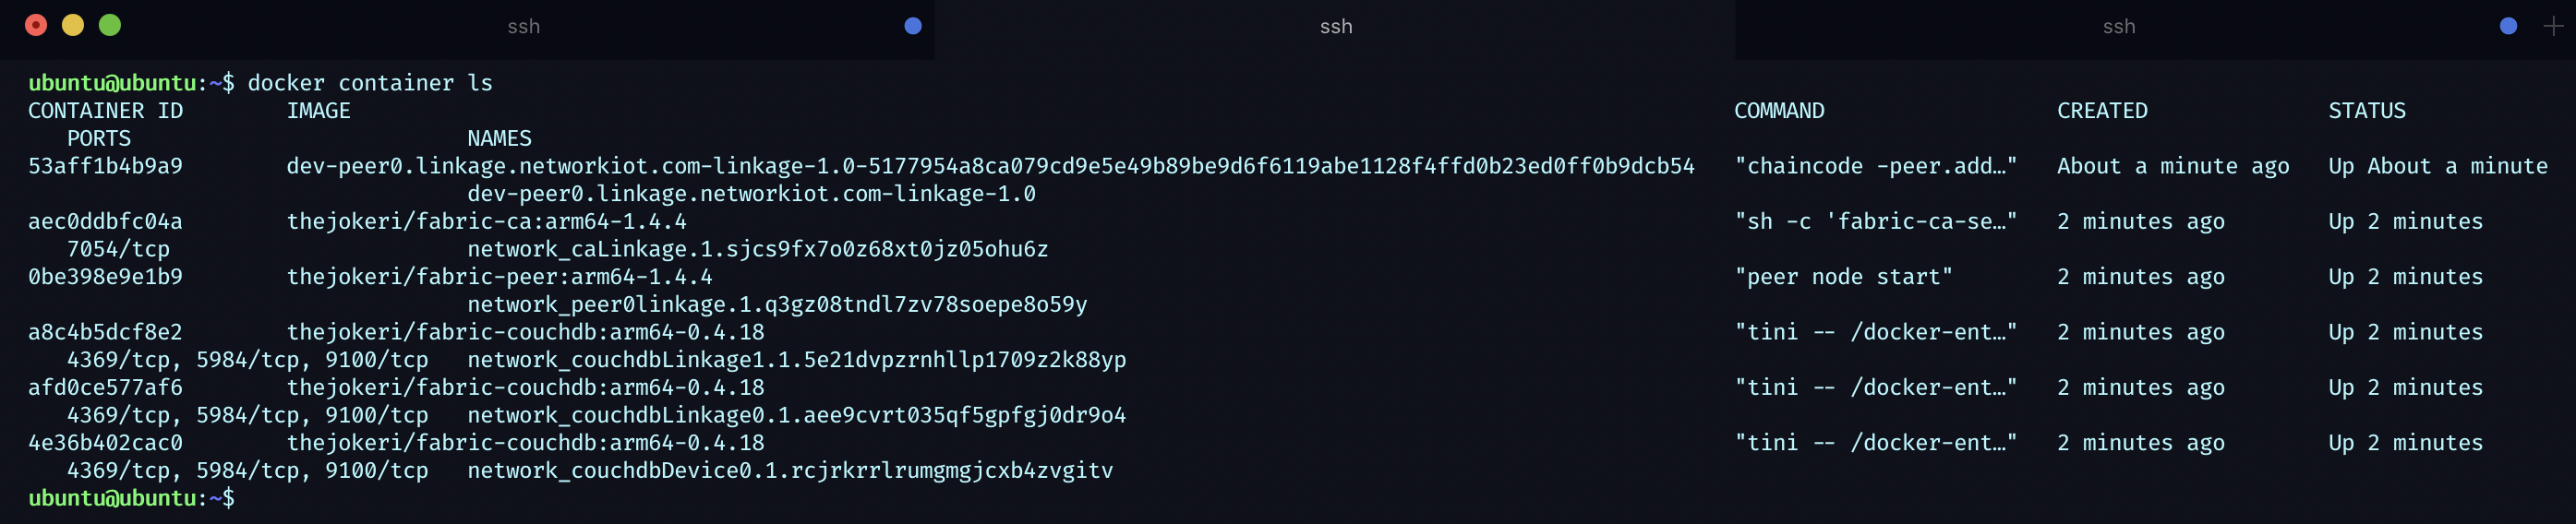
\includegraphics[width=\textwidth]{imagenes/desarrollo/comandos/containers_worker1}
  \caption{Salida de contenedores en el nodo worker 1.}
  \label{fig:containers-worker1}
\end{figure}

\begin{figure}[ht!]
  \centering
  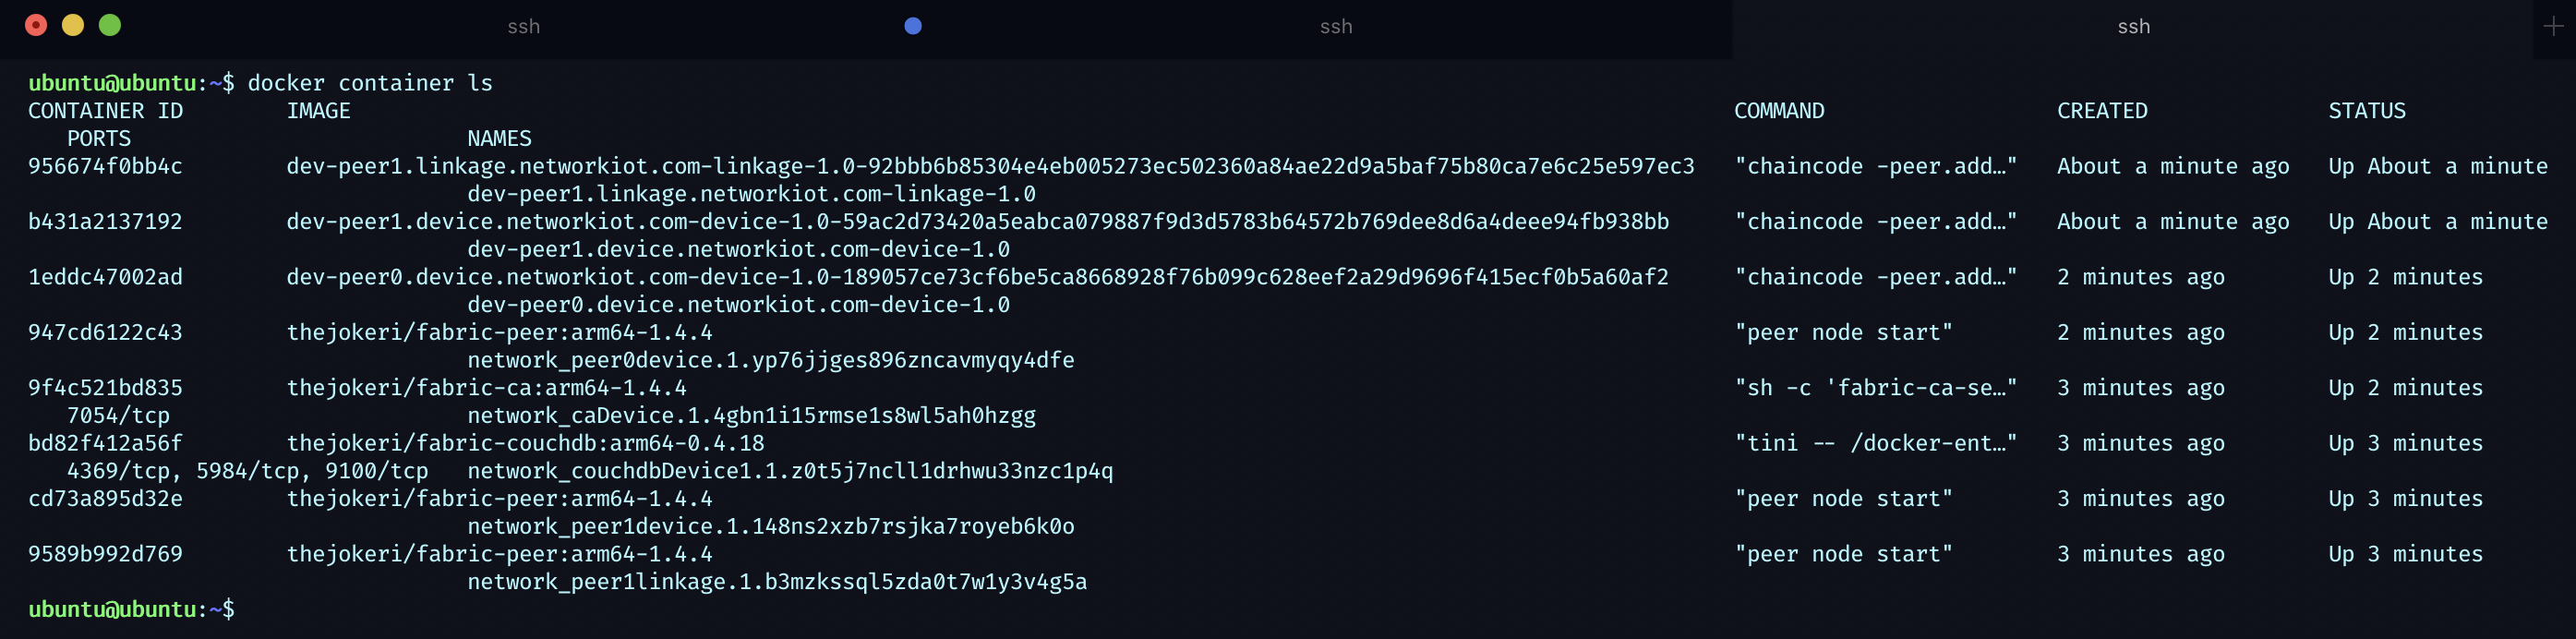
\includegraphics[width=\textwidth]{imagenes/desarrollo/comandos/containers_worker2}
  \caption{Salida de contenedores en el nodo worker 2.}
  \label{fig:containers-worker2}
\end{figure}

\noindent El comando \textbf{remove} se encargará de eliminar toda la configuración de la red Blockchain y eliminará los 
contenedores y servicios creados.

\begin{figure}[ht!]
  \centering
  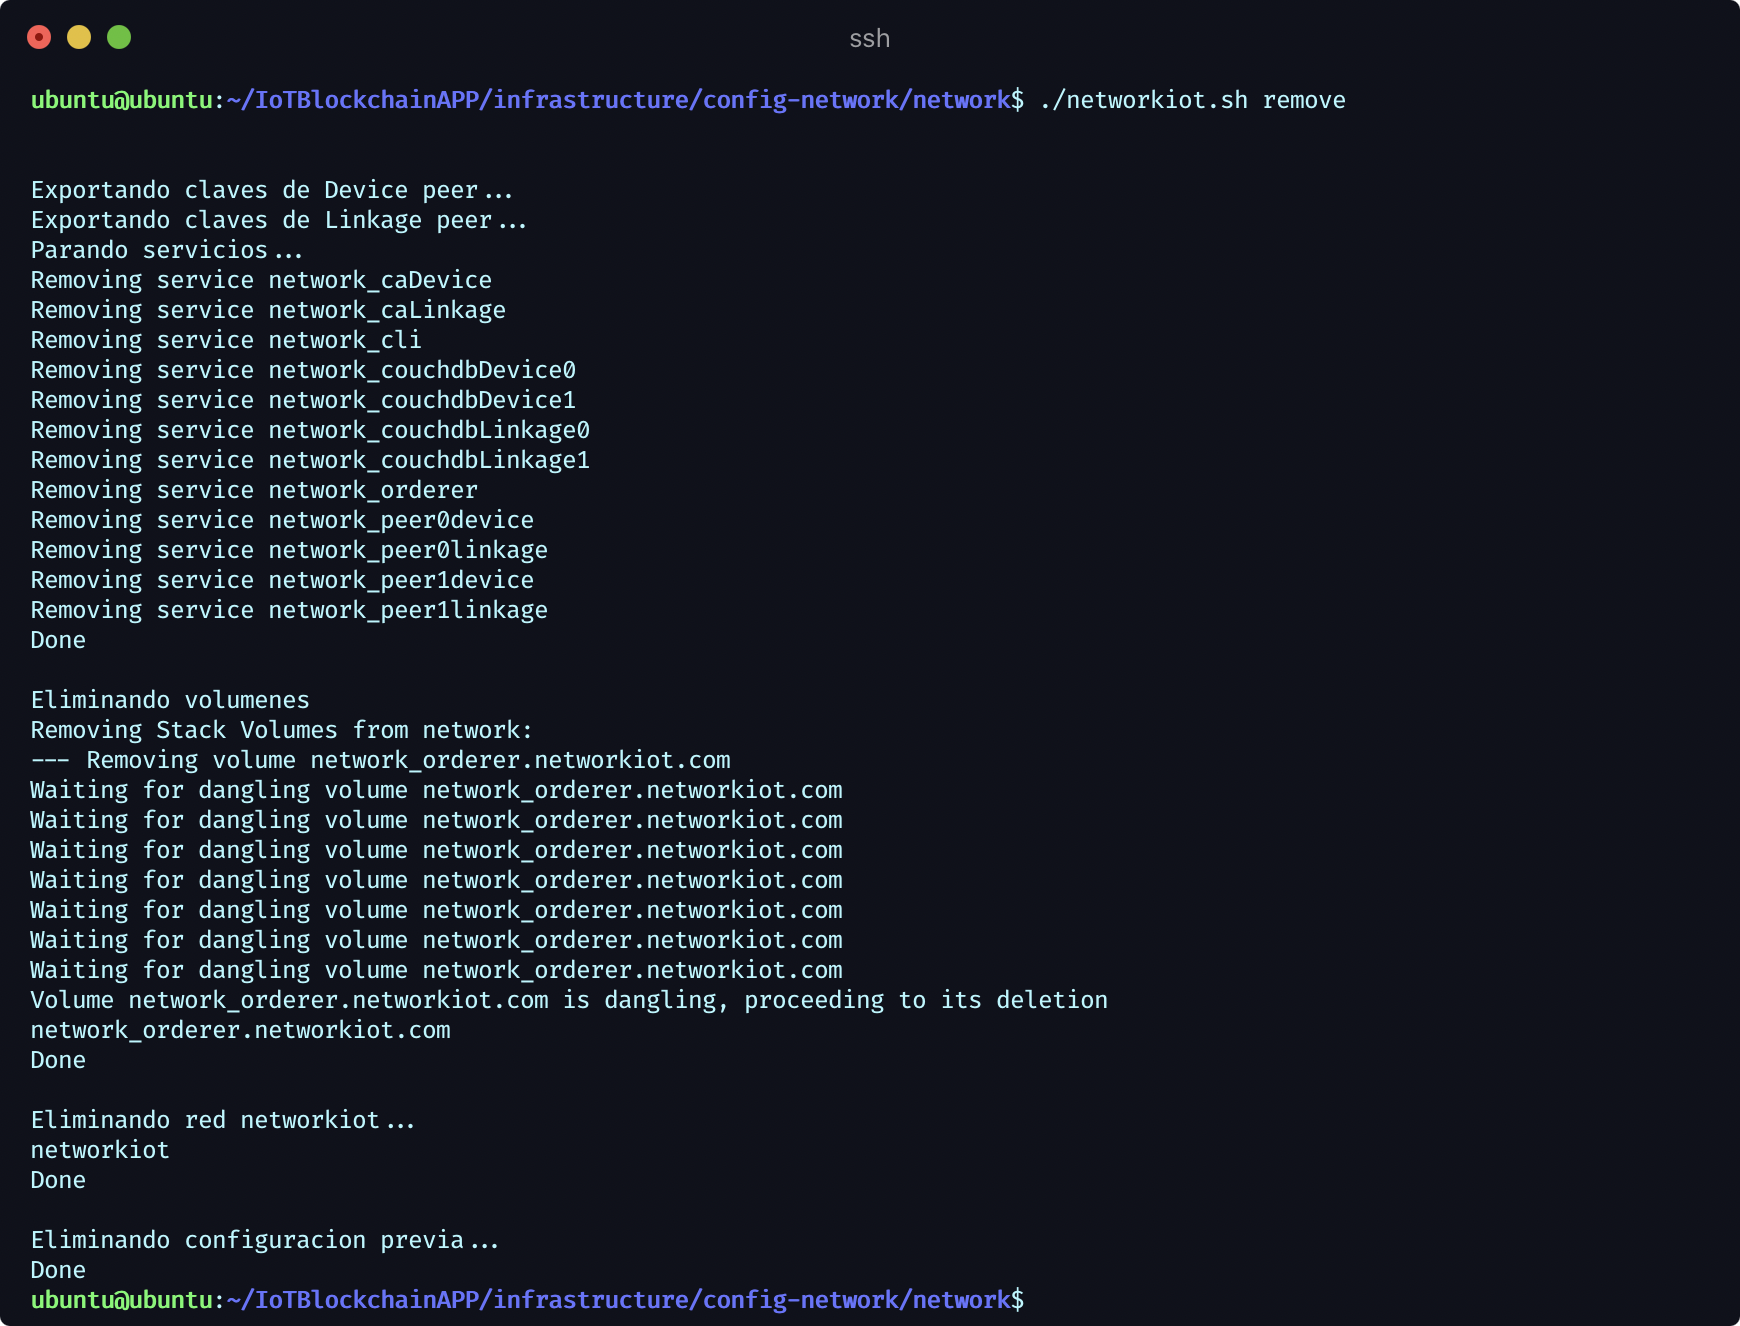
\includegraphics[width=0.8\textwidth]{imagenes/desarrollo/comandos/remove}
  \caption{Opción remove del script networkiot.}
  \label{fig:remove}
\end{figure}

\subsection{Desarrollo del Back end.}

En este capítulo, se mencionará la arquitectura del lado del servidor utilizando GraphQL, Apollo Server y Express, 
implementado con Node.js. Se utilizará el SDK de Hyperledger Fabric para realizar consultas y mantener un registro 
en la red Blockchain \cite{documentation-home-apollo-basics, express-docs, hyperledger-fabric-node-sdk}. La API 
consta de tres partes esenciales: Models, Resolvers y Schemas. Además de un apartado de config para la creación y 
gestión de usuarios y una carpeta utils para realizar la conexión directa a la red Blockchain \cite{structure-graphql-node.js} 
(ver fig. \ref{fig:tree-server}).

\begin{figure}[ht!]
  \centering
  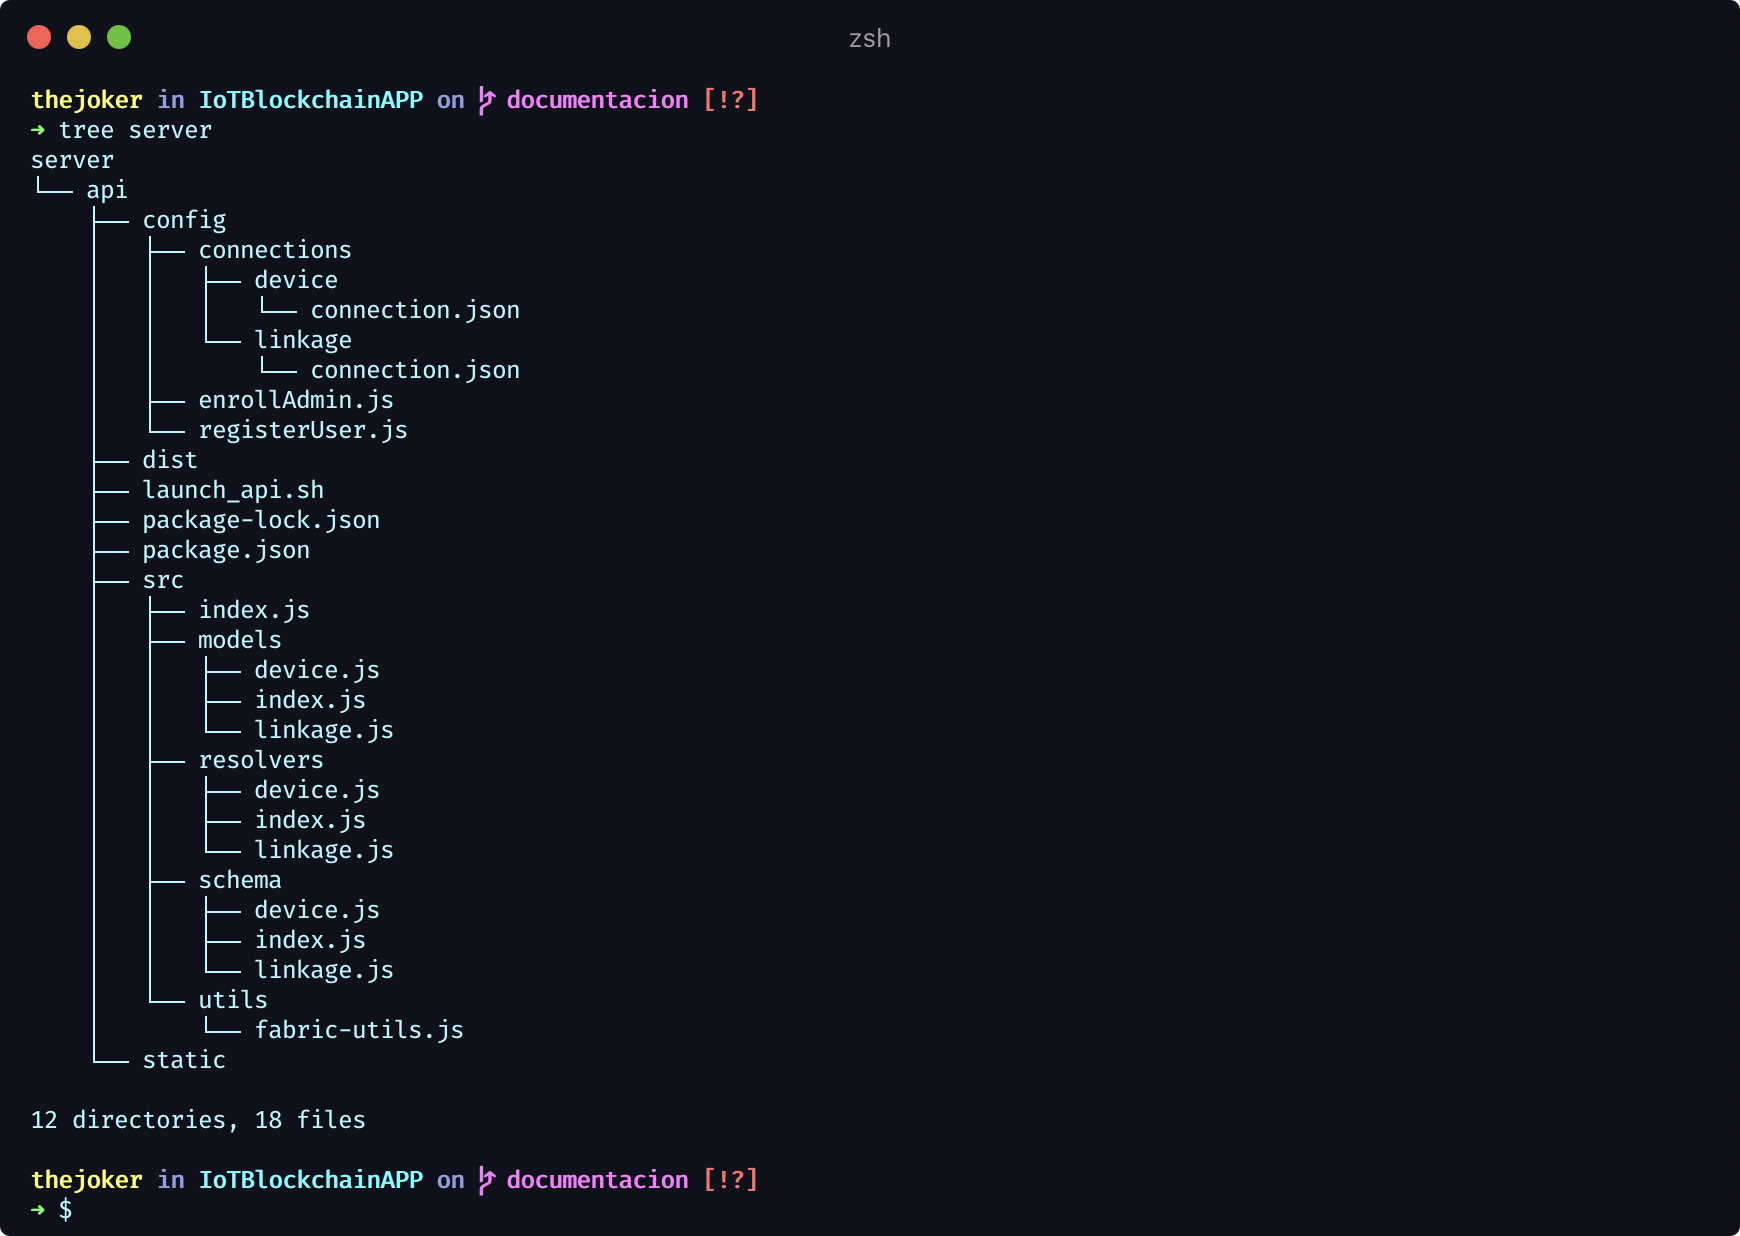
\includegraphics[width=\textwidth]{imagenes/desarrollo/tree_server}
  \caption{Tree de la carpeta server.}
  \label{fig:tree-server}
\end{figure}

\noindent Los Schemas en GraphQL se define por sus tipos, las relaciones entre los tipos y su estructura. Por lo 
tanto, GraphQL utiliza un lenguaje de definición de esquemas (SDL). Sin embargo, el esquema no define de dónde 
provienen los datos. Esta responsabilidad es manejada por los Resolvers que se encargán de obtener los datos desde la 
red Blockchain. Son ellos, los que se encargan de mandar las peticiones para crear, consultar, actualizar y/o borrar 
\cite{hyperledger-fabric-couchdb}. Y por último, los Models son los encargados de manejar esas queries y formatear los 
datos recibidos en forma de objectos, aplicando el paradigma de orientado a objetos \cite{graphql-server-tutorial, 
thinking-graphs}.

\vspace{5mm}

\noindent Con la herramienta de GraphQL Playground, podemos realizar consultas directamente a la API y nos permite 
mostrar la documentación y los Schemas de la misma. Permite una ayuda durante el desarrollo y además elaborar 
documentación sobre la API. (ver fig. \ref{fig:graphql-api}, \ref{fig:query-graphql-api}, \ref{fig:graphql-docs}, 
\ref{fig:graphql-schema}).

\vspace{5mm}

\noindent Para permitir conexiones por HTTPS en el lado del servidor, se ha utilizado Let's Encrypt y Certbot, una 
herramienta de EFF, conocido como Electronic Frontier Foundation, la principal organización sin ánimo de lucro centrada 
en la privacidad, la libertad de expresión y las libertades civiles en general en el mundo digital. Con ella podemos 
generar certificados SSL con la herramienta Certbot. Y Con Express indicamos la lectura de ficheros estáticos para 
permitir que se ejecute bajo HTTPS \cite{setup-lets-encrypt}. 

\vspace{5mm}

\noindent Para llevarlo acabo, es necesario establecer un dominio, por ello he utilizado la herramienta NO-IP, para crear 
dominios bajo DDNS. En el router se establece el DDNS indicando el nombre del dominio y se abre los puertos 80 y 443, para 
permitir conexiones HTTP y HTTPS. Todas las conexiones se redireccionan al servidor maestro (192.168.0.30).

\vspace{5mm}

\noindent Una vez creado el dominio, se creará tres ficheros: key.pem, cert.pem y chain.pem. Hacemos que Express lea los 
ficheros y cree el servidor bajo el puerto 443 y cualquier otra conexión por el puerto 80, sea redireccionada. Con ello 
hemos conseguido que la API sea accesible desde fuera y que tenga conexiones seguras.

\vspace{5mm}

\noindent Para levantar el servidor en el nodo maestro, he creado un script \textbf{launch\_api.sh} que se va a ocupar de 
copiar los archivos de crypto-config, instalar las dependencias del package.json, inscribir al usuario admin, userDevice y 
userLinkage y comenzar el servicio escuchando por el puerto 443. 

\begin{figure}[ht!]
  \centering
  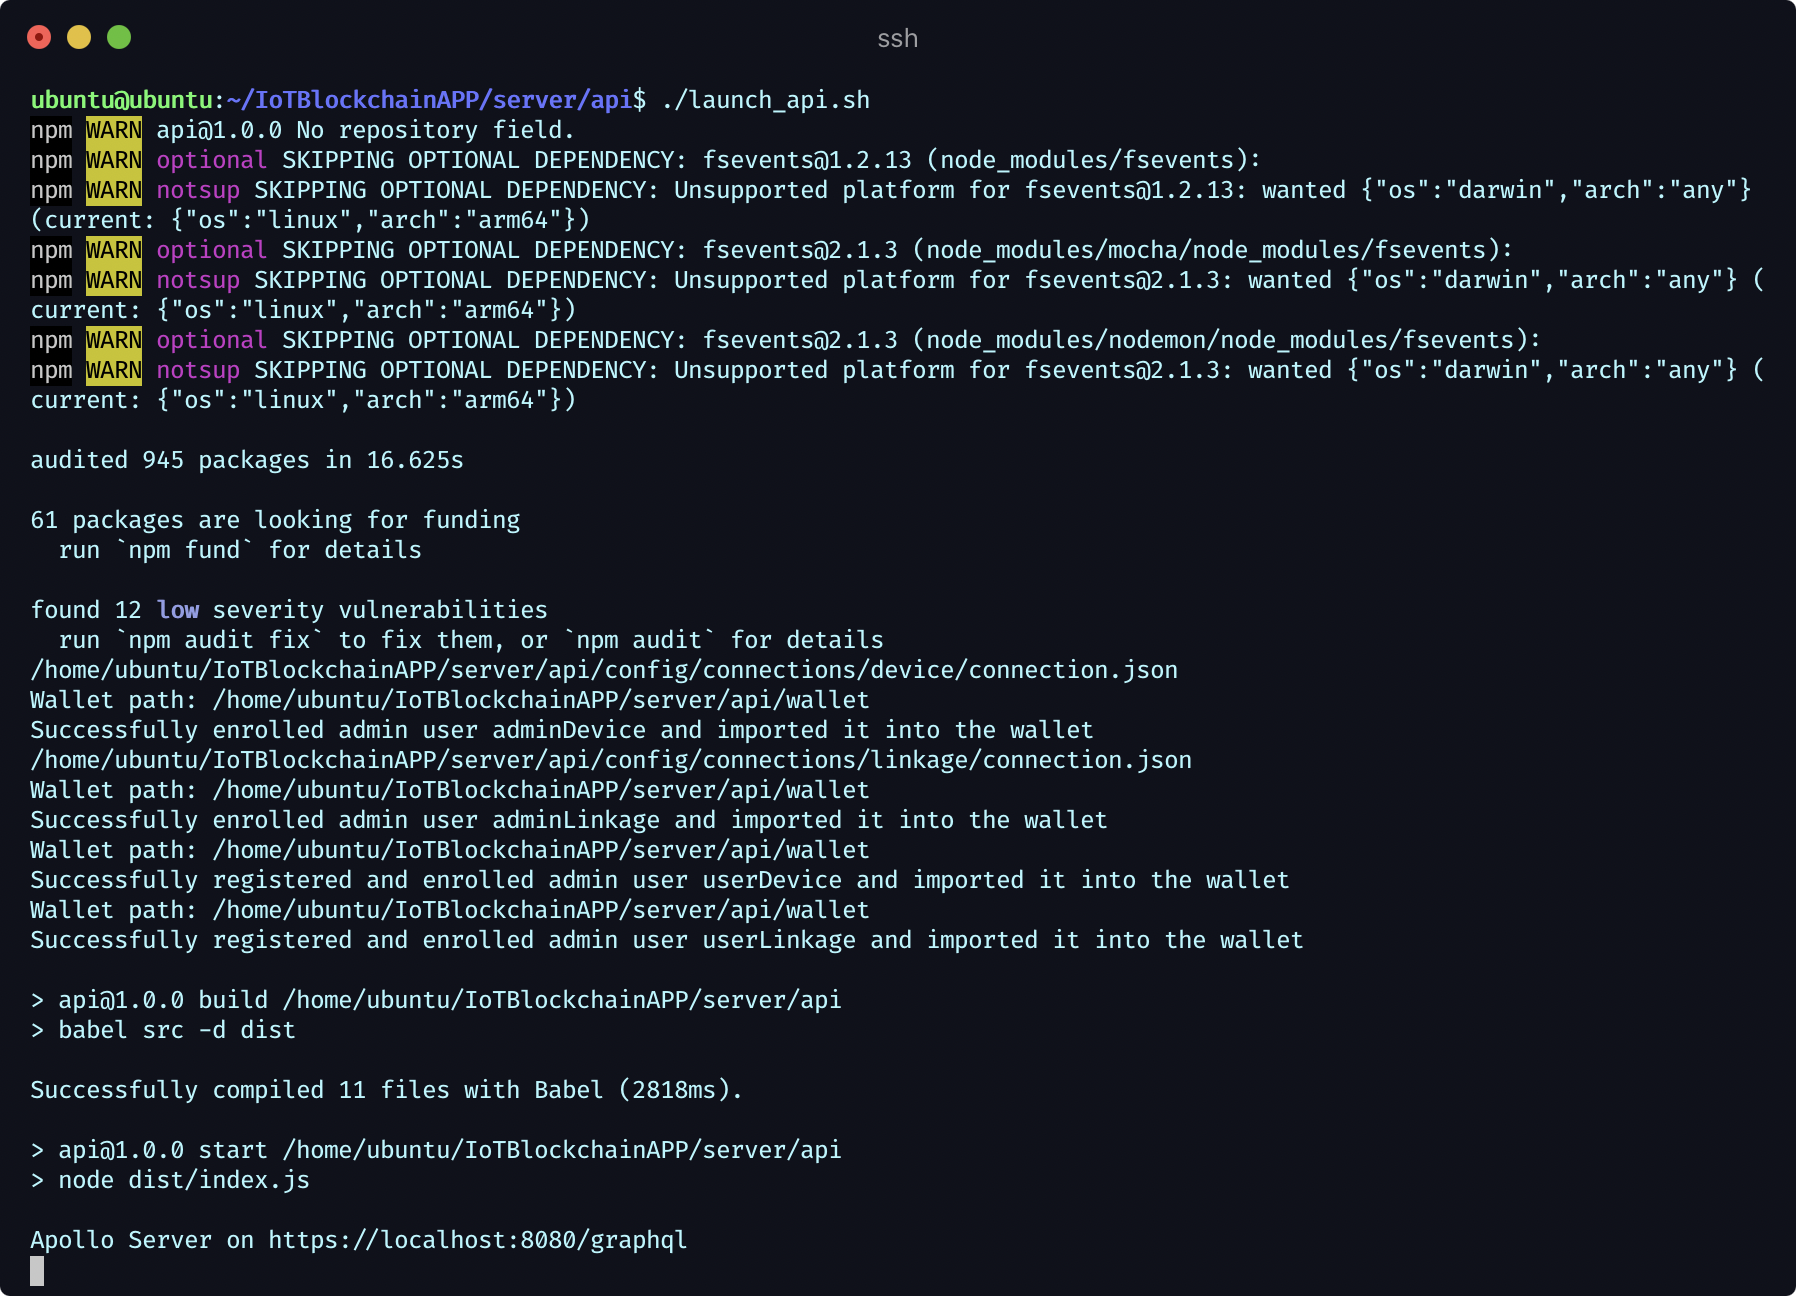
\includegraphics[width=0.7\textwidth]{imagenes/desarrollo/comandos/launch_api}
  \caption{Ejecución del script launch\_api.}
  \label{fig:launch-api}
\end{figure}

\subsection{Desarrollo del Front end y despliegue.}

Para elaborar la interfaz del usuario, he utilizado Gatsby.js que es un generador de sitios web estáticos para 
aplicaciones React, y soportado por Apollo Client. Gatsby producirá archivos HTML estáticos precargados de antemano, 
lo cual permite renderizar la interfaz muy rápidamente. Una de las ventajas que tiene Gatsby, es que utiliza GraphQL para 
realizar las consultas y por tanto, es un candidato perfecto para la API elaborada 
\cite{react, introduction-apollo-client}.

\vspace{5mm}

\noindent También tiene un rico ecosistema de plugins, que para este proyecto he utilizado el plugin de PWA, en el que 
hay que indicar un manifiesto, añadir el plugin de offline y trabajar bajo HTTPS
\cite{progressive-web-app-gatsby, gatsby-manifest, gatsby-offline}. 

\vspace{5mm}

\noindent Para que Gatsby pueda trabajar de forma dinámica, se ha configurado la interfaz para realizar consultas
a la API con Apollo Client \cite{setup-apollo-gatsby}. Además de crear una utilidad que permite renderizar tablas 
dependiendo de los datos que reciba \cite{dynamic-table}.

\begin{figure}[ht!]
  \centering
  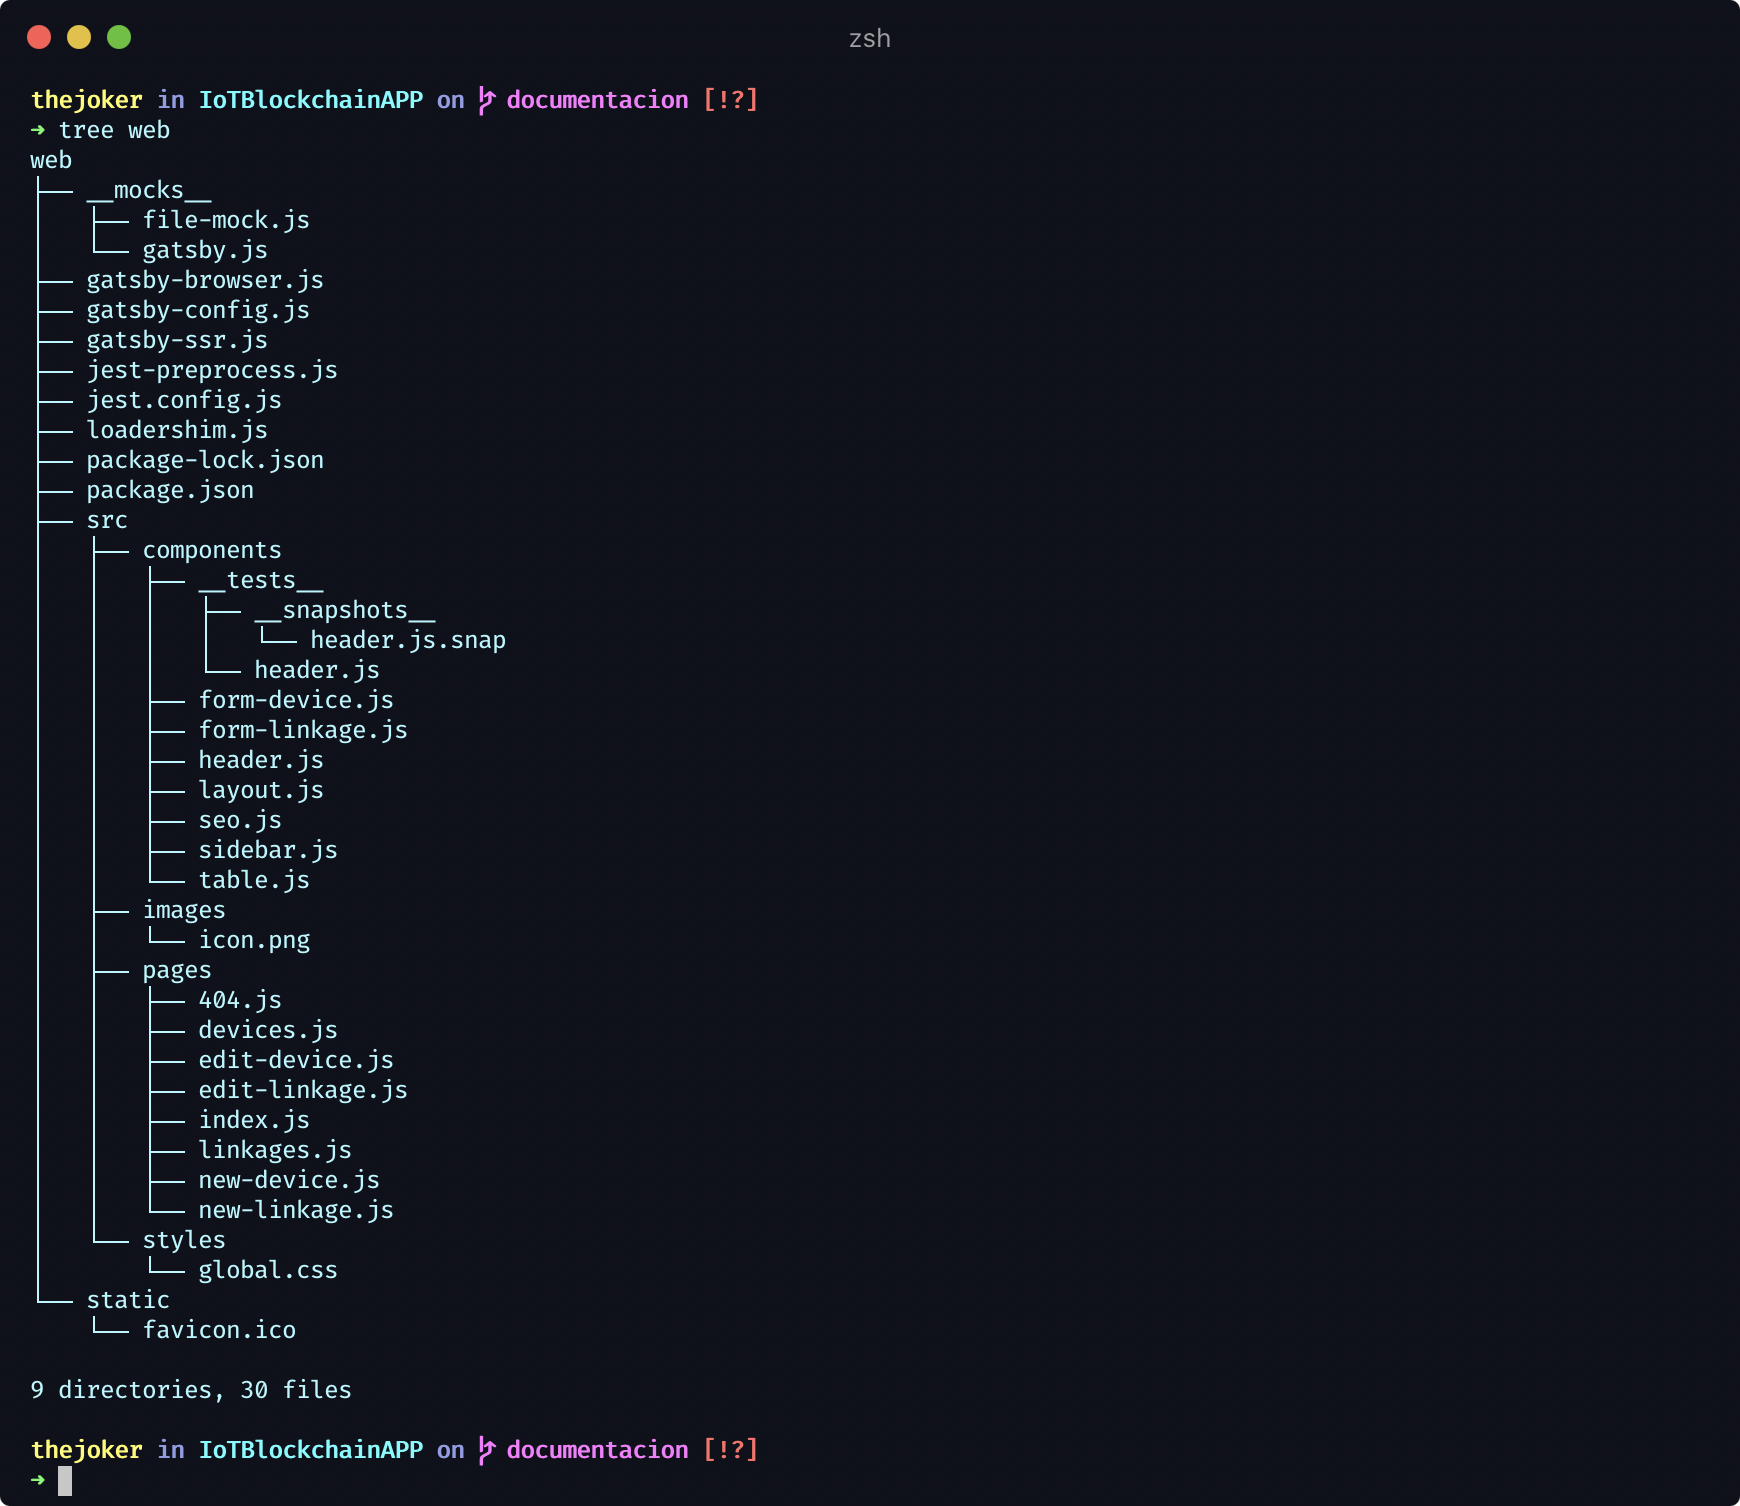
\includegraphics[width=\textwidth]{imagenes/desarrollo/tree_web}
  \caption{Tree de la carpeta web.}
  \label{fig:tree-web}
\end{figure}

\vspace{5mm}

\noindent Cabe destacar, que se ha llevado a cabo test unitarios, para comprobar que se renderiza bien la interfaz de 
usuario, además de vincular el repositorio con Continious Integration (CI), para que en cada actualización que se realice 
en el código, se lancen los test antes de desplegarlo en Gatsby Cloud \cite{unit-test, travis-ci-nodejs}.

\vspace{5mm}

\noindent Finalmente, la arquitectura de la aplicación y de la infraestructura se puede ver en la siguiente figura
y las URL son: 

\begin{itemize}
  \item https://iotblockchainapp.gtsb.io/ (Front end)
  \item https://iotblockchainapi.ddns.net/ (Back end)
\end{itemize}

\begin{figure}[ht!]
  \centering
  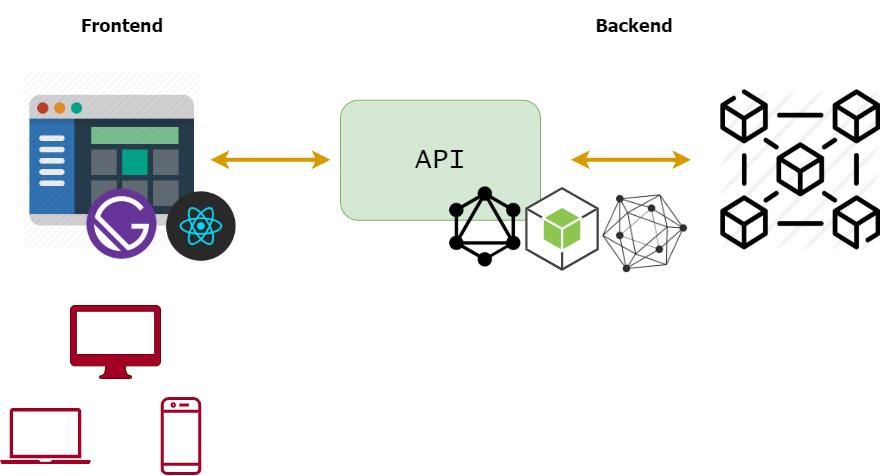
\includegraphics[width=\textwidth]{imagenes/desarrollo/arquitectura_aplicacion}
  \caption{Arquitectura de la aplicación.}
  \label{fig:arquitectura-aplicacion}
\end{figure}

\newpage